\documentclass[12pt,a4paper]{scrreprt}

\usepackage{cmap}
\usepackage[T1]{fontenc} 
\usepackage[utf8]{inputenc}
\usepackage[english,russian]{babel}

\usepackage{caption}
\usepackage{subcaption}
\usepackage[normalem]{ulem}

%\usepackage{soulutf8}

\usepackage{float}

\usepackage{enumitem}

\usepackage{graphicx}
\usepackage{multirow}


\usepackage{pgfplots}
\pgfplotsset{compat=newest}
\usepgfplotslibrary{units}


\usepackage{caption}
\captionsetup{labelsep=endash}
\captionsetup[figure]{name={Рисунок}}
\captionsetup[subfigure]{name={Рисунок}}
\captionsetup[subtable]{labelformat=simple}
\captionsetup[subfigure]{labelformat=simple}
\renewcommand{\thesubtable}{\text{Таблица }\arabic{chapter}\text{.}\arabic{table}\text{.}\arabic{subtable}\text{ --}}
%\renewcommand{\thesubfigure}{\arabic{chapter}\text{.}\arabic{figure}\text{.}\azbuk{\subfigure}\text{ --}}


\usepackage{textcomp}
\usepackage{chngcntr}

\usepackage{amsmath}
\usepackage{amsfonts}
\usepackage{array}

\usepackage{geometry}
\geometry{left=10mm}
\geometry{right=10mm}
\geometry{top=10mm}
\geometry{bottom=10mm}
\geometry{foot=1.7cm}

\usepackage{listings}
\lstset{ %
	language=haskell,                 % выбор языка для подсветки (здесь это С)
	basicstyle=\small\sffamily, % размер и начертание шрифта для подсветки кода
	numbers=left,               % где поставить нумерацию строк (слева\справа)
	numberstyle=\tiny,           % размер шрифта для номеров строк
	stepnumber=1,                   % размер шага между двумя номерами строк
	numbersep=5pt,                % как далеко отстоят номера строк от подсвечиваемого кода
	showspaces=false,            % показывать или нет пробелы специальными отступами
	showstringspaces=false,      % показывать или нет пробелы в строках
	showtabs=false,             % показывать или нет табуляцию в строках
	frame=single,              % рисовать рамку вокруг кода
	tabsize=2,                 % размер табуляции по умолчанию равен 2 пробелам
	captionpos=t,              % позиция заголовка вверху [t] или внизу [b] 
	breaklines=true,           % автоматически переносить строки (да\нет)
	breakatwhitespace=false, % переносить строки только если есть пробел
	escapeinside={\#*}{*)}   % если нужно добавить комментарии в коде
}


\usepackage{titlesec}
\titleformat{\section}
{\normalsize\bfseries}
{\thesection}
{1em}{}
\titlespacing*{\chapter}{0pt}{-30pt}{8pt}
\titlespacing*{\section}{\parindent}{*4}{*4}
\titlespacing*{\subsection}{\parindent}{*4}{*4}
\titlespacing*{\subsubsection}{\parindent}{*4}{*4}

%\renewcommand\thesubfloat{(\roman{subfloat})}
\renewcommand\thesubfigure{(\asbuk{subfigure})}

% Маркировка для списков
\def\labelitemi{$\circ$}
\def\labelitemii{$*$}
\usepackage{pdflscape}

\usepackage{setspace}
\onehalfspacing % Полуторный интервал

\captionsetup[table]{skip=0pt,singlelinecheck=off, justification=raggedleft}
\captionsetup[table]{skip=0pt,singlelinecheck=off, justification=centering}

\frenchspacing
\usepackage{indentfirst} % Красная строка

\usepackage{titlesec}
\usepackage{xcolor}
% Названия глав
\titleformat{\section}{\huge\textmd}{\thesection}{1em}{}

\definecolor{gray35}{gray}{0.35}

\titleformat{\chapter}[hang]{\Huge}{\textcolor{gray35}{\thechapter. }}{0pt}{\huge\scshape}

\titleformat{\section}{\Large}{\textcolor{gray35}\thesection}{20pt}{\Large\scshape}
\titleformat{\subsection}{\large}{\thesubsection}{20pt}{\large\scshape}
\titleformat{\subsubsection}{\large}{\thesubsubsection}{20pt}{\large\scshape}

\newcommand*{\undertext}[2]{%
	\begin{tabular}[t]{@{}c@{}}%
		#1\\\relax\scriptsize(#2)%
	\end{tabular}
}

\emergencystretch 10em

% Настройки введения

\addtocontents{toc}{\setcounter{tocdepth}{3}}
\addtocontents{toc}{\setcounter{secnumdepth}{3}}

\usepackage{tocloft,lipsum,pgffor}

\addtocontents{toc}{~\hfill\textnormal{Страница}\par}

\renewcommand{\cftpartfont}{\normalfont\textmd}

\addto\captionsrussian{\renewcommand{\contentsname}{Содержание}}
\renewcommand{\cfttoctitlefont}{\Huge\textmd}

\renewcommand{\cftchapfont}{\normalfont\normalsize}
\renewcommand{\cftsecfont}{\normalfont\normalsize}
\renewcommand{\cftsubsecfont}{\normalfont\normalsize}
\renewcommand{\cftsubsubsecfont}{\normalfont\normalsize}

\renewcommand{\cftchapleader}{\cftdotfill{\cftdotsep}}

\usepackage{listings}
\usepackage{pdflscape}
\usepackage{everypage}
\usepackage{xcolor}

%\bibliographystyle{gost780u.bst}
%
%\usepackage[backend=biber,
%%			bibencoding=utf8,
%%			sorting=nyt,
%%			maxcitenames=2,
%			style=gost-numeric-min,
%%			autolang=other, 
%%			natbib=true,
%%			maxnames=99,
%			uniquename=false]{biblatex}

\usepackage{csquotes} 
\usepackage[backend=biber,
			style=gost-numeric,
			maxcitenames=3,
			maxbibnames=12,
			minnames=1,
			movenames=false,
			ibidtracker=false,
			sorting=none,
			autolang=other]{biblatex}
			
\DeclareSourcemap{
	\maps[datatype=bibtex]{
		\map{
			\step[fieldsource=langid, match=russian, final]
			\step[fieldset=presort, fieldvalue={a}]
		}
		\map{
			\step[fieldsource=langid, notmatch=russian, final]
			\step[fieldset=presort, fieldvalue={z}]
		}
	}
}

\addbibresource{ref-lib.bib} % База библиографии

\usepackage[pdftex]{hyperref} % Гиперссылки
\hypersetup{hidelinks}

% Листинги 
\usepackage{listings}

\definecolor{darkgray}{gray}{0.15}

\definecolor{teal}{rgb}{0.25,0.88,0.73}
\definecolor{gray}{rgb}{0.5,0.5,0.5}
\definecolor{b-red}{rgb}{0.88,0.25,0.41}
\definecolor{royal-blue}{rgb}{0.25,0.41,0.88}



% какой то сложный кусок со стак эксчейндж для квадратных скобок
\makeatletter
\newenvironment{sqcases}{%
	\matrix@check\sqcases\env@sqcases
}{%
	\endarray\right.%
}
\def\env@sqcases{%
	\let\@ifnextchar\new@ifnextchar
	\left\lbrack
	\def\arraystretch{1.2}%
	\array{@{}l@{\quad}l@{}}%
}
\makeatother

% и для матриц
\makeatletter
\renewcommand*\env@matrix[1][\arraystretch]{%
	\edef\arraystretch{#1}%
	\hskip -\arraycolsep
	\let\@ifnextchar\new@ifnextchar
	\array{*\c@MaxMatrixCols c}}
\makeatother

\usepackage{pdflscape}
\usepackage{fancyhdr} 

\fancypagestyle{mylandscape}{
	\fancyhf{} %Clears the header/footer
	\fancyfoot{% Footer
		\makebox[\textwidth][r]{% Right
			\rlap{\hspace{.75cm}% Push out of margin by \footskip
				\smash{% Remove vertical height
					\raisebox{6in}{% Raise vertically
						\rotatebox{90}{\thepage}}}}}}% Rotate counter-clockwise
	\renewcommand{\headrulewidth}{0pt}% No header rule
	\renewcommand{\footrulewidth}{0pt}% No footer rule
}


\begin{document}
	
\thispagestyle{empty}
\begin{titlepage}
	\normalsize
	\noindent \begin{minipage}{0.15\textwidth}
		
\includegraphics[width=\linewidth]{pics/logo}
	\end{minipage}
	\noindent\begin{minipage}{0.9\textwidth}\centering
		\textbf{Министерство науки и высшего образования Российской Федерации}\\
		\textbf{Федеральное государственное бюджетное образовательное учреждение высшего образования}\\
		\textbf{~~~«Московский государственный технический университет имени Н.Э.~Баумана}\\
		\textbf{(национальный исследовательский университет)»}\\
		\textbf{(МГТУ им. Н.Э.~Баумана)}
	\end{minipage}
	
	\noindent\rule{18cm}{3pt}
	\newline
	\noindent ФАКУЛЬТЕТ $\underline{\text{«Информатика и системы управления»}}$ \newline
	\noindent КАФЕДРА $\underline{\text{«Программное обеспечение ЭВМ и информационные технологии»}}$\newline\newline\newline\newline\newline
	
	\begin{center}
		\noindent\begin{minipage}{1.3\textwidth}\centering
			\Large\textbf{Конспект лекций и семинаров}\newline
			\textbf{по курсу}\newline
			\textbf{<<Операционные системы>>, 2 семестр}\newline
		\end{minipage}
	\end{center}
	
	~\\\\\\\\\\\\\\
	\normalsize
	\noindent\textbf{Студент } $\underline{\text{Сироткина П.Ю.}}$\newline\newline
	\noindent\textbf{Группа } $\underline{\text{ИУ7-66Б}}$\newline\newline
	\noindent\textbf{Преподаватель } $\underline{\text{Рязанова Н.Ю.}}$\newline
	
	\begin{center}
		\vfill
		Москва~---~\the\year
		~г.
	\end{center}
\end{titlepage}
	
\tableofcontents

\setcounter{tocdepth}{2}
	
\chapter{\textbf{Семинар №1. 10 февраля 2022}}

\chapter{\textbf{Лекция №1. 19 февраля 2022}}

\section{Файловая подсистема Linux}

Файловая система предназначена для обеспечения возможности хранения и доступа к файлам в системе.

Файл (рабочий) - информация, хранимая во вторичной памяти или во вспомогательном ЗУ с целью ее сохранения после завершения отдельного задания или преодоления ограничений, связанных с объемом основного ЗУ.

Файл - любая поименнованная совокупность данных, которая хранится во вторичной памяти.

Файловая система - порядок, определяющий способ организации, хранения, именования и доступа к данным на вторичных носителях информации.

Любая ФС имеет иерархическую структуру, это связано с разными уровнями ФС, т.к. различные задачи, которые ей решаются, выполняются на разных уровнях ОС. Именование файлов (символьный уровень) - самый высокий уровень ФС. Он позволяет пользователю в удобной форме задавать имена файлов и искать их в каталогах

Обобщенная модель ФС: файл хранится на физическом устройстве, причем в системе такое устройство внешнее, значит на нижнем уровне доступ к файлу осуществляется через подсистему ввода-вывода, т.е. для того, чтобы считать файл необходимо обратиться к внешнему устройству.

Иерархическая структура ФС:

\begin{figure}[!h]
	\center{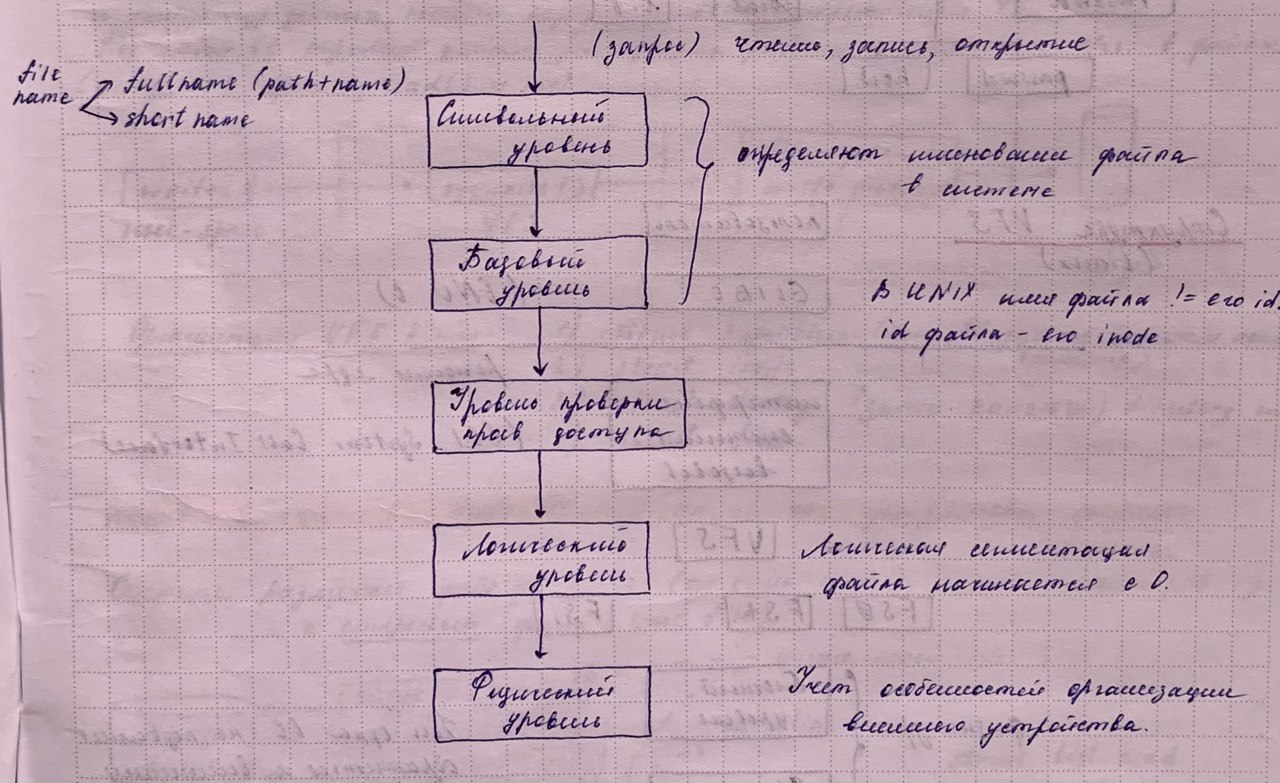
\includegraphics[scale=0.41]{pics/fs.jpg}}
\end{figure}

Полное имя = путь к файлу + имя файла. В UNIX путь начинается с корневого каталога. Права доступа RWX. 

В данном случае файл похож на программу. Любая программа считает, что она начинается с 0-ого адреса, т.е. в программе находится смещение. Логическая организация файла начинается с 0.

Бинарный файл - это блочный файл. Текстовый файл - это символьный файл. Типы файлов характеризуют операции над ними. Для блочного файла характерна возможность обращения к некому блоку (fseek), для текстового - наличие символа конца файла.

Это связано с тем, что ОС поддерживает 2 типа устройств (символьные и блочные). 2 типа потоков передачи данных: байто-ориентированные и блоко-ориентированные. Дисковые устройства и флэш-память - единственные блочные устройства. Все остальные устройства - символьные.

ФС UNIX организована через интерфейс VFS/vnode. В Linux не определена vnode, только VFS. Задача vnode - ОС без изменений ядра могла поддерживать большое кол-во самых разных ФС.

\begin{figure}[!h]
	\center{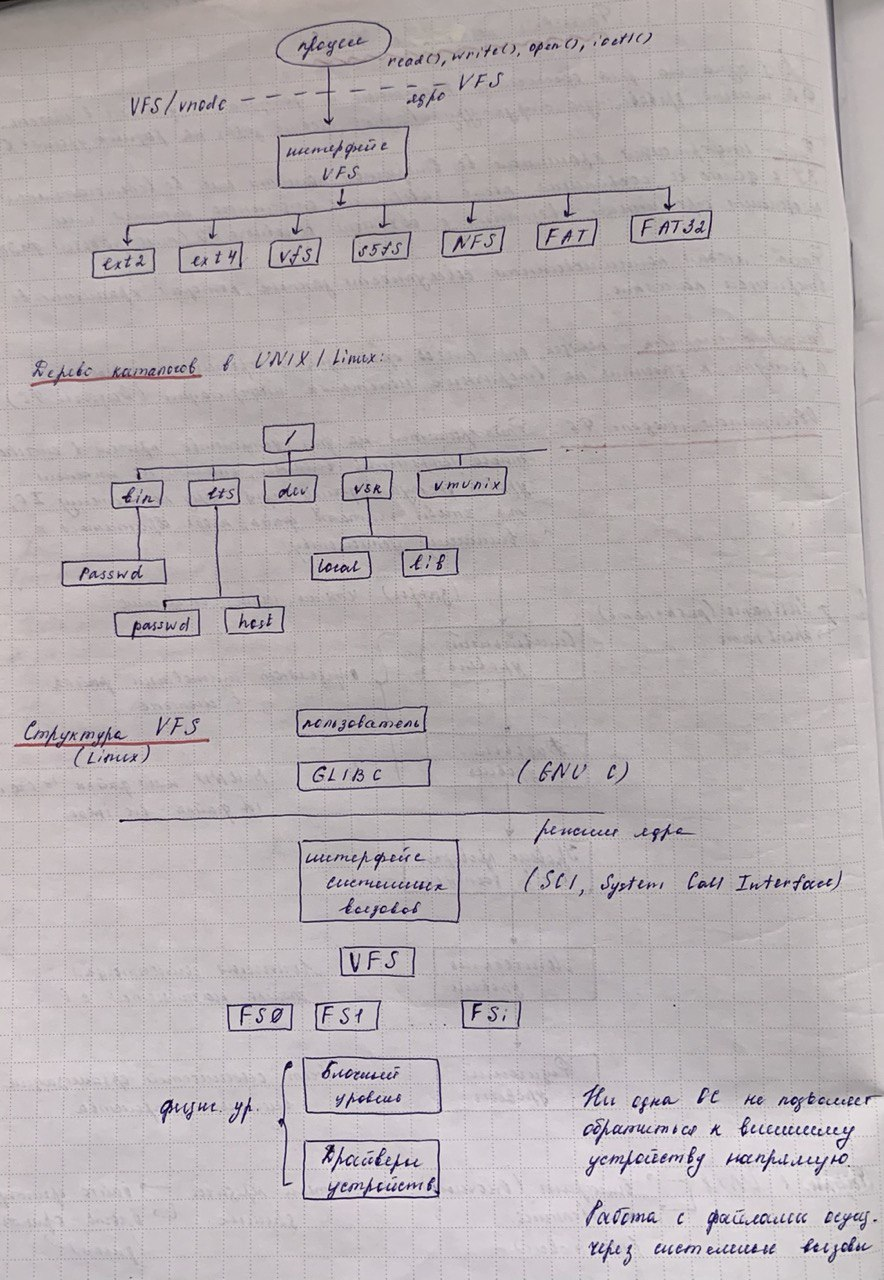
\includegraphics[scale=0.35]{pics/fs2.jpg}}
\end{figure}

Демонстрация особенностей физического уровня:

\begin{figure}[!h]
	\center{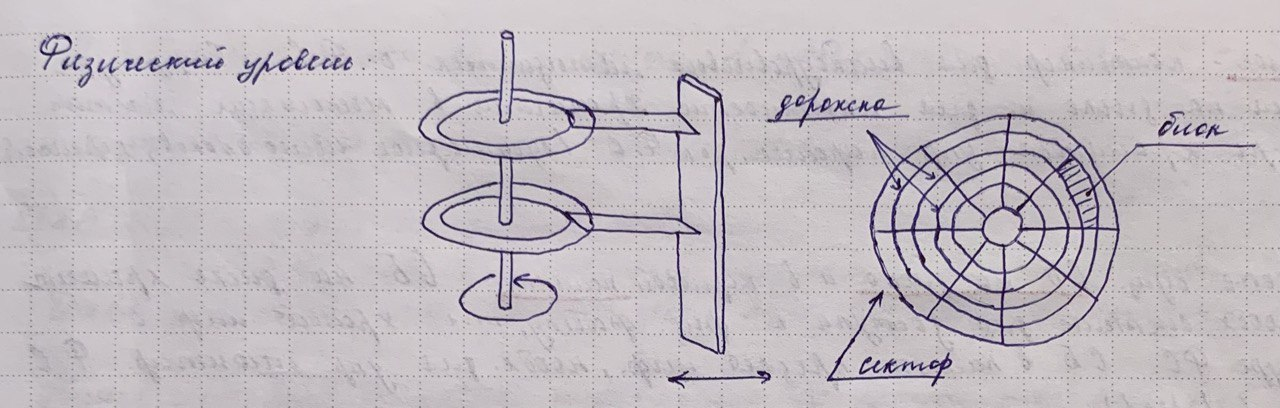
\includegraphics[scale=0.35]{pics/fs3.jpg}}
\end{figure}

В дисках дорожки - концентрические окружности. Совокупность дорожен одного радиуса состоляет цилиндр. Также они разделены на сектора. При этом мы знаем, что жесктий диск постоянно вращается и имеется считывающая/записывающая головка, которая перемещается поступательно, для того чтобы получить доступ к блоку на определенной дорожке.

Современные ФС поддерживают т.н. очень большие файлы. Проводится аналогия с управлением памятью страницами по запросу. Это означает, что любая страница адресного пространства процесса может быть загружена в любую страницу физической памяти. Для того, чтобы управлять этим, существуют таблицы страниц. Аналогично современные ФС обеспечивают хранение файлов вразброс, т.е. файл не занимает на диске непрерывную последовательность адресов. Это обеспечивается хранением адресов блоков. <<Родная ФС>> - ext2.

Возможность поддержки большого количества разных ФС реализуется засчет того, что в состав системы входит слой абстракции над собственным низкоуровневым интерфейсом ФС. Для этого ВФС предоставляет общую файловую модель, которая способна отображать общие возможности и поведение любой возможной ФС. 

Такой уровень абстракции работает на основе базовых концептуальных интерфейсов и структур данных, которые поддерживаются конкретными ФС. Фактически код любой ФС скрывает детали реализации непосредственной работы с данными, организованными в файлы, а именно предоставляют пользователю набор API, таких как открыть файл, прочить, удалить и т.д. В любом варианте любая ФС поддерживает такие понятия как файл, каталог, и действия, определенные над ними.

Это можно представить следующей абстракцией:

\begin{figure}[!h]
	\center{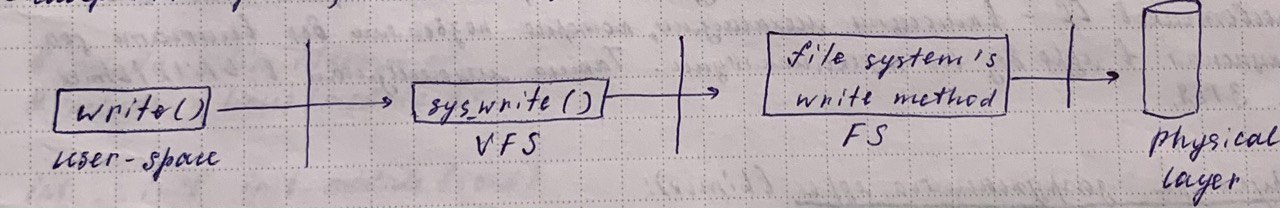
\includegraphics[scale=0.35]{pics/fs4.jpg}}
\end{figure}

ВФС предоставляет общую файловую модель, которая наследует ФС, реализуя действия для различных posix api. 

Как видно, системный вызов write() сначала обрабатывается общим системным вызовом sys\_write(), которая	определяет фактический способ записи файлов, характерный для такой ФС, на которой находится файл. Затем общий системный вызов sys\_write() вызывает метод конкретной ФС, чтобы выполнить запись данных на физический носитель. Т.е. ВФС скрывает особенности работы с конкретным физическим устройством.

Внутренняя организация VFS Linux:

\begin{itemize}
	\item struct superblock (описывает ФС, расположенную на внешнем носителе);
	\item struct inode (индексный узел);
	\item struct dentry (запись каталога, dentry = directory entry);
	\item struct file.
\end{itemize}

\begin{figure}[!h]
	\center{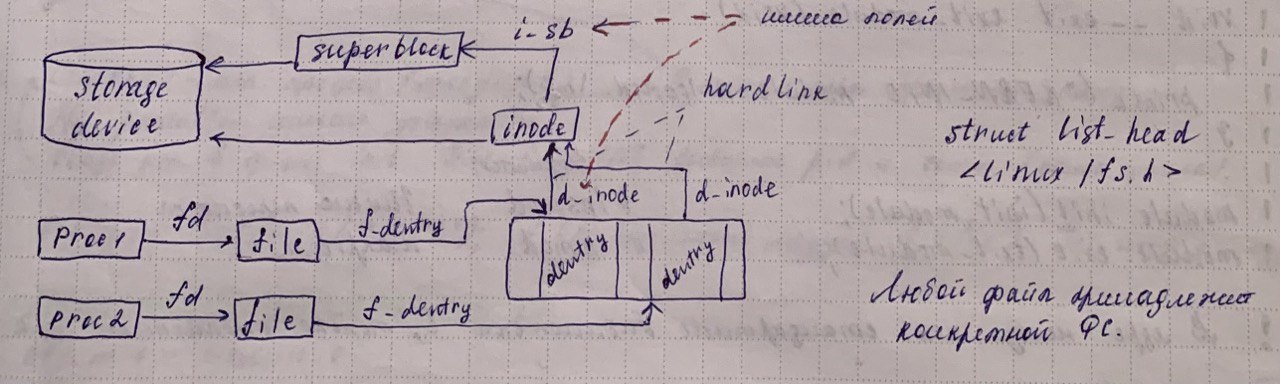
\includegraphics[scale=0.35]{pics/fs5.jpg}}
\end{figure}

Два процесса открывают один и тот же файл. Чтобы обеспечить к нему доступ, имеется dentry (обеспечивает работу с каталогами).

Система различает файл, находящийся на диске (его описывает struct inode) и открытый файл (его описывает struct file). i\_sb, d\_inode - не идентификаторы, а имена полей соответствующих структур.

Структура superblock в ВФС описывает конкретную подмонтированную ФС, т.е. ФС, которая располагается на внешнем носителе.

Суперблок - контейнер для высокоуровневых метаданных о ФС. Структура находится на диске и для надежности хранится в нескольких местах. В структуре хранятся управляющие параметры ФС (такие как суммарное число блоков, свободное число блоков, корневой inode и т.д.).

В системе существует суперблок на диске и суперблок в оперативной памяти. Суперблок на диске хранит информацию, необходимую системе для доступа к физическому файлу, т.е. хранит информацию о структуре ФС. Суперблок в памяти предоставляет информацию, необходимую для управления смонтированной ФС (struct list\_head, связный список суперблоков, <linux/fs.h>).

Монтирование - система действий, в результате которой ФС устройства становится доступной, т.е. можно получить доступ к информации, которая хранится на устройстве.

\begin{lstlisting}
	mount keys -t fs_type -o options_fs device catalog
\end{lstlisting}

\chapter{\textbf{Семинар №2. 24 февраля 2022}}

\chapter{\textbf{Лекция №2. 5 марта 2022}}

\chapter{\textbf{Семинар №3. 10 марта 2022}}

\chapter{\textbf{Лекция №3. 19 марта 2022}}

\chapter{\textbf{Семинар №4. 24 марта 2022}}

\chapter{\textbf{Лекция №4. 2 апреля 2022}}

\chapter{\textbf{Семинар 7 апреля 2022}}

\chapter{\textbf{Лекция 16 апреля 2022}}

\section{Структура dentry}

Ранее рассмотрели структуру dentry, которая описывает элемент пути, начиная с корневого каталога (со слэша). 

Эта структура хранится в библиотеке <linux/dcach.h>. При этом в этом кэше кэшируются inode-ы, которые представляют элементы пути. Любой элемент пути/директория - это файл. Кэширование делается для того, чтобы сократить время доступа к файлам. Все данные, к которым мы обращаемся, кэшируются.

Если человек обратился к какому-либо файлу, наиболее вероятно, что он обратится к нему еще раз. На этом принципе (LRU) строится кэширование. Пользователь не может ждать неопределенно долго. Время ответа системы не должно превышать 3 секунд.

Обратимся к следующему файлу: /home/dracula/src/foo.c. Для того, чтобы система обратилась к файлу foo.c, необходимо, чтобы она <<спустилась>> по всем элементам пути.

Каждый такой элемент каталога - специальный файл, иначе невозможно хранить информацию об дереве каталогов, которое позволяет получить доступ к каталоговым файлам. Т.е. каждый такой элемент каталога будет иметь реальный inode, но эти элементы каталога с точки зрения структуры dentry создаются на лету.

Кэш объектов dentry состоит из:

\begin{enumerate}
	\item Список используемых объектов dentry, которые связаны с определенным inode. В struct inode находится поле i\_dentr. Поскольку один и тот же inode может иметь несколько ссылок, соотвующих директориям, то это поле должно представлять из себя связный список.
	\item Двусвязный список неиспользуемых и негативных объектов dentry по алгоритму LRU, т.е. в списке находятся объекты dentry, к которым были последние обращения. Добавление в этот список нового объекта dentry должно выполняться по значению времени. Если происходит обращение в объекту dentry, он переносится в хвост. Новый объект dentry записывается в хвост. Удаление элементов выполняется из головы как наиболее долго находящийся в списке, к нему наиболее долго не было обращение. 
	
	LRU здесь используется в чистом виде, в отличие от LRU для страниц. Обращение к странице выполняется очень часто, на каждой команде, а то и несколько раз, причем в этой команде м.б. косвенная адресация, значит надо было бы каждый раз редактировать список LRU. Это очень большие накладные расходы. В случае файлов нет такого дикого кол-ва обращений.
	\item Хэш-таблица (dentry\_hash\_table) и хэш-функция, которые позволяют преобразовать заданный путь в объект dentry. Каждый элемент этой таблицы (массива) является указателем на список тех объектов dentry, которые соответствуют какому-то ключу. Значение ключа определяется функцией d\_hash(), что позволяет для каждой ФС реализовать свою хэш-функцию. Поиск в хэш-таблице осуществляется функцией d\_lookup().
\end{enumerate}

Приведенный пример показывает, что сначала идет поиск в dentry\_cach, если поиск приводит к тому, что какого-то элемента каталога нет в этом кэше, то тогда производится обращение таким образом, который мы рассмотрели. В результате найденный объект dentry (его inode) будет помещен в кэш.

Структура dentry имеет указатель на dentry\_operations, рассмотрим эту структуру.

\begin{lstlisting}
struct dentry_operations
{
	...
	int (*d_hash)(const struct dentry *, struct qstr *);
	int (*d_compare)(const struct dentry *, const struct dentry *, 
												unsigned int, const char *, const struct qstr *);
	int (*d_delete)(const struct dentry *);
	...
	struct vfsmount *(*d_automount)(struct path *);
	...
};
\end{lstlisting}

\section{Кэш inode (слаб)}

Есть dentry cach, но dentry не исчерпывает всех потребностей. В linux inode cach находится в файле fs/inode.c. 

Inode cach представляет из себя:

\begin{enumerate}
	\item Глобальный хэш-массив inode\_hashtable(), в котором каждый inode хэшируется по значению указателя на суперблок и номеру inode. 
	
	В случае отсутствия суперблока (inode\_i\_sb == NULL) вместо хэш-массива inode добавляется к двусвязному списку anon\_hash\_chain. Пример таких анонимных inode: сокеты, которые создаются функцией sock\_alloc() (<net/socket.c>), которая вызывает функцию get\_empty\_inode() из <fs/inode.c>.
	\item Глобальный список inode\_in\_use, содержит inode, у которых i\_count > 0 и i\_nlink > 0. Inode-ы, созданные с помощью вызова функций get\_empty\_inode() и get\_new\_inode(), добавляются в этот список.
	\item Глобальный список inode\_unused, содержит правильные/допустимые inode, для которых i\_count = 0.
	\item Также для каждого суперблока имеется sb$\rightarrow$dirty - список грязных inode (i\_count > 0 и i\_nlink > 0, но они помечены как модифицированные, т.е. как i\_dirty). Такой грязный inode добавляется в список sb$\rightarrow$dirty, если он кэширован. Это позволяет синхронизировать работу с inode.
	\item Slab cache, который называется inode\_cachep. Динамический (slab) кэш, в нем inode могут освобождаться, создаваться, вставляться и изыматься. 
\end{enumerate}

Все перечисленные списки защищены спин-локом inode\_lock(). 

Слаб - <<брусок>>, имеющий определенный размер. Подход был введен для OS SUN. 

Идея: в ядре значительные объемы памяти выделяются на ограниченный и определенный набор объектов, таких как дескрипторы файлов, inode и т.д. При этом время для создания каждого такого объекта по меркам системы является значительным. 

В результате для каждого такого объекты выполняется выделение памяти; когда объект уже становится не нужным, то выполняется освобождение объекта. При интенсивной работе в системе эти объекты постоянно создаются и освобожадются - это трата времени.

Поэтому, если такой объект был и создан и в нем на некоторое время отпала нужда, тем не менее не удалять его из памяти, то есть оставить соответствующий объем памяти, занимаемый объектом, причем оставить в проинициализированном состоянии, для того, чтобы в последующем этот проинициализированный объект использовать для объектов этого же типа.

(Спрашивает на экзамене про семафоры и мьютексы по отношению к слаб кэшу).

Главные структуры слаб-распределителя:

\begin{figure}[!h]
	\center{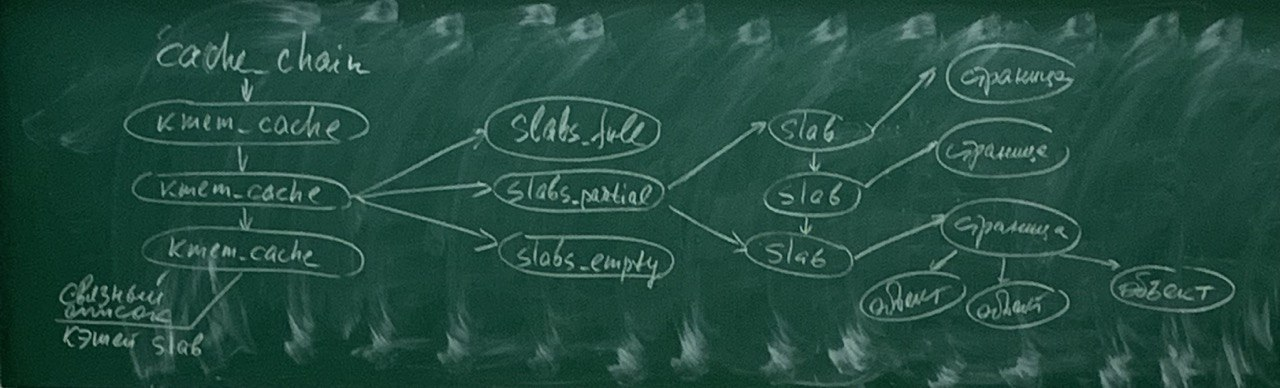
\includegraphics[scale=0.41]{pics/slab.jpg}}
\end{figure}

Связный список нужен для агоритма best\_fit - самый подходящий, т.е. ищет кэш более всего соответстсвующий размеру нужного рапсределения.

Виды слабов:

\begin{itemize}
	\item slab\_full - распределен полностью;
	\item slab\_partial - распределен частично;
	\item slab\_empty - пустой, основной кандидат на reaping(возвращение для дальнейшего использования).
\end{itemize}

Объекты - основные элементы, которые выделяются из соответствующего кэша и возвращаются в него.

В реализации слабов участки памяти, подходящие для размещения объектов данных определенного размера и типа, определяются заранее. Распределитель (аллокатор) слабов хранит информацию о размещении этих участков, которые также известны как кэш. В результате, если возникает запрос на выделение памяти определенного размера, то он удовлетворяется быстро.

Существует библиотека <linux/slab.h>. ВФС proc предоставляет информацию о слабе: cat /proc/slabinfo.

Функции для работы со слабом:

\begin{lstlisting}
struct kmem_cache *kmem_cache_create(const char *name, size_t size, size_t offset, unsigned long  flags, void (*ctor)(void *));

int kmem_cache_destroy(kmem_cache_t *cache);

void *kmem_cache_alloc(kmem_cache_t *cache, int flags);

void *kmem_cache_free(kmem_cache_t *cache, const void *obj);
\end{lstlisting}

\section{Структура FILE}

Эта структура описывает т.н. открытые файлы, т.е. структура предоставляет информацию системе о файлах, которые были открыты процессами. Это одна единственная таблица, недоступная пользователю.

Для процесса открытия файла в различных структурах, даже в структурах ядра, имеется функция open. Мы говорим об обычных (regular) открытых файлах.

Работа этой структуры в системе начинается, когда какой-то файл открывается. Чтобы открыть файл в своих программах, мы вызываем системный вызов open. Сейчас мы говорим о режиме пользователя.

Библиотека <fcntl.h>:

\begin{lstlisting}
int open(const char *pathname, int oflags, .../* mode_t *mode */);

fd = open("myfile", O_RDWR | O_CREATE | O_EXCL, 0644);
\end{lstlisting}

Флаг O\_CREATE предписывает, что если файл не существует, то необходимо его создать. И этот флаг требует в обязательном порядке наличие следующего аргумента: mode.

Флаг O\_EXCL предписывает, что если флаг (файл?) уже существует, но задан флаг O\_CREATE, возникла ошибка. 

Такая комбинация флагов позволяет выполнять проверку существования файла и его создание атомарно.

Системный вызов open возвращает файловый дескриптор.

\chapter{\textbf{Семинар 21 апреля 2022}}

\section{Буфферизованный/небуфферизованный ввод-вывод (открытые файла)}

ЛР дает понимание, с какими функциями мы имеем дело, поскольку функции ввода-вывода могут быть буфферизованные (библиотека stdio), а функции read, write, open - функции небуферизованного ввода-вывода. Работа в режиме пользователя.

Именно обычные файлы предназначены для долговременного хранения информации.

Традиционно программирование изучается под UNIX.

Начнем со структуры task\_struct, поскольку файлы открывают процессы.

\begin{lstlisting}[language=C]
struct task_struct 
{
	... 
	/* File System Information*/
	struct fs_struct *fs;
	... 
	/* Open File Information*/
	struct files_struct *files;
	...
	/*namespaces*/
	struct nsproxy *nsproxy;
}

struct nsproxy 
{
	atomic_t count;
	struct uts_namespace *uts_ns;
	struct ipc_namespace *ipc_ns;
	struct mnt_namespace *mnt_ns; //Previously only it
	struct pid_namespace *pid_ns;
	struct net *net_ns;
}
\end{lstlisting}

В современных UNIX-системах 5 namespace-ов. Дальше эту тему мы не развиваем.

Любой процесс когда-то был файлом, пока мы его не запустили на выполнение. Любой файл принадлежит определенной ФС. Когда файл открывается (системный вызов open или библиотечная функция fopen), в системе создается т.н. открытый файл, т.е. создается структура struct\_file для этого файла в одной единственной таблице открытых файлов, содержащей дескрипторы всех открытых файлов в системе, в том числе файлов, открытых в ядре. Это таблица принадлежит ядру и не доступна пользователю.

Любая структура - это таблица. Соответственно, struct\_file является дескриптором открытого файла.

Рассмотрим структуры:

\begin{lstlisting}[language=C]
struct fs_struct
{
	int users;
	spinlock_t lock;
	seg_amount seg;
	int umask;
	int in_exec;
	struct path, root, pwd; //Root and current dir
}

struct path 
{
	struct ufsmount *mnt;
	struct dentry *dentry;
}
\end{lstlisting}

Следующая структура описывает файлы, открытые процессом (не более 64 файлов).
\begin{lstlisting}[language=C]
struct files_struct
{
	...
	unsigned int next_fd; //amount of open by process files, next
	unsigned long close_on_exec_init();
	unsigned long open_fds_init();
	struct file rcu *fd_array[NR_OPEN_DEFAULT]; //Constant - amount of open files
}
\end{lstlisting}

Поле close\_on\_exec\_init(): указывает Число файлов, которые должны быть закрыты системным вызовом exec
 
Поле open\_fds\_init(): определяет число открытых файлов.

RCU - Real Compute Unit. 

Поле fd\_array - двумерный массив файловых объектов (массив указателей на struct file). Принято созданные системой открытые файлы по аналогии с другими структурами называть объектами, т.е. это экземпляр структуры struct\_file, открытый файл.

Ни Unix, ни Linux не имеют отношение к ООП, они написаны на С.

Важно: exec - переводит процесс на новое адрессное пространство программы, которое переданно exec-у в качестве параметра. Процесс при этом не создается, он тот же, но в результате начинает выполняться другая программа, и ей не нужны файлы, которые были октрыты до того, как она начала выполняться.

\begin{lstlisting}[language=C]
struct file
{
	...
	struct path f_path;
	struct inode *f_inode;
	const struct file_operations *f_ops; //Defines ops on concrete open file.
	atomic_long_t f_count;
	unsigned int f_flags;
	fmode_t f_mode; //Access mode
	...
	lofft_t f_pos;//Important
}
\end{lstlisting}

Когда процесс открывает файл, f\_pos = 0 (нулевое смещение, начало файла).

Демонстрируемая проблема: разные процессы могут открывать один и тот же файл с одним и тем же inode, но они могут иметь разные имена. Один и тот же файл открывается несколько раз. В этом случае необходимо понимать, что может возникнуть при неправильной работе с данными. Также рисуем схему взаимодействия структур ядра.

Свяжем эти структуры:

\begin{figure}[!h]
	\center{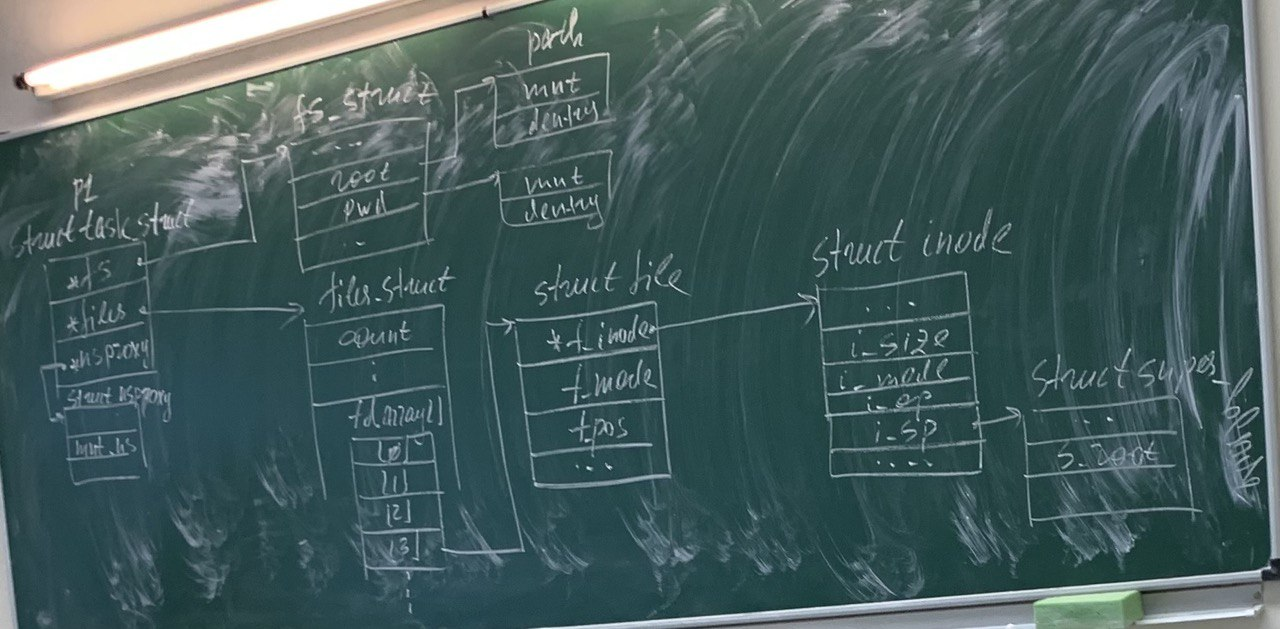
\includegraphics[scale=0.41]{pics/buf_schema.jpg}}
\end{figure}

Для любого процесса будут открыты потоки stdin, stdout, stderr (0, 1, 2 на схеме). Файлы, открытые программистом, будут начинаться с индекса 3. Каждый элемент этого массива ссылается на struct file. Нас интересуют файлы, открываемые open и fopen.

Фактически данная связь структур отличает программы, использующие open. С fopen добавляется еще одна структура. Чтобы получить дескриптор, определяем struct \_\_IO\_FILE (<stdio.h>). В этой структуре определены поля, связанные с буфером. 

(Эта структура есть в отчете к ЛР)

\begin{lstlisting}[language=C]
struct __IO_FILE
{	
	...
	char *__IO_buf_base;
	char *__IO_buf_end;
	...
	int __fileno;
}
\end{lstlisting}

Поля: fileno - указатель на дескриптор открытого файла процесса, индекс в массиве десрипторов открытых файлов процесса.

Библиотека stdio - библиотека буфферизованного ввода-вывода. Если мы осуществляем запись в файл, то сначала информация записывается в буфер вывода. Если мы читаем информацию из файла, то сначала информация записывается в буфер чтения. Это создает дополнительные проблемы при работе с файлами, особенно когда один и тот же файл открывается несколько раз в одно и то же время.

Ситуации, при которых содержимое буфера переписывается в файл:

\begin{itemize}
	\item Буфер заполнился;
	\item Вызов функции fflash;
	\item Вызов функции fclose.
\end{itemize}

Система автоматически закрывает часть файлов, если мы не указали fclose.

Одновеременный доступ разных процессов к одному и тому же файлу является источником проблем, которые получили название raise condition(гонки). 

Рассмотрим следующую ситуацию: пусть 2 процесса открывают один и тот же файл в режиме read/write. Один процесс добавляет запись в конец файла, для этого он сначала вызывает fseek, но вызывать функцию write не успевает, т.к. переходит в состояние сна, т.е. теряет квант. Второй процесс делает аналогичные действия, чтобы записать информацию в конец файла. Ему это удается и он переходит к другой работе. Первый процесс пробуждается, продолжает выполнять указанные действия, т.е. он уже получил позицию, в которой должен записать данные в файл. Он выполняет запись, в результате он запишет свои данные поверх данных, которые записал второй процесс. Т.е. данные потеряны.

Решение: необходимо использовать неделимый (atomic) системный вызов, которым является системный вызов в режиме O\_APPEND для open. Если этот режим установлен, то каждой операции append гарантируется неделимость.

Следующая ЛР: связана с системным вызовом open, предполагает создание алгоритма выполнения системного вызова open, т.е. это работа с функциями и структурами ядра. В open всегда вызываетс sys\_open, который реализован в виде switch. Т.е. в результате вызова ситема переходит из режима пользователя в режим ядра. Вызов open может открыть существующий файл, а может создать новый. Если создается новый, должен быть создан inode. При одних флагах идет обращение к файлу, а при других создание inode, это целый ряд вызовов функций ядра.

\chapter{\textbf{Лекция 30 апреля 2022}}

\section{Прерывания}

Основа работы ОС - система прерываний. В монолитном ядре все построено на прерываниях. В настоящее время принято выделять:

\begin{enumerate}
	\item Системные вызовы.
	\item Исключения.
	\item Аппаратные прерывания.
\end{enumerate}

Когда говорят о прерываниях(nterrupts), то речь идет об аппаратных прерываниях. 

Основную группу прерываний состовляют прерывания от устройств ввода-вывода. Без этих устройств пользоваться вычислительной системой невозможно, т.к. именно эти устройства предназначены для взаимодействия с пользователем. 

При этом аппаратные прерывания от внешних устройств возникают, когда внешнее устройство \textit{завершило} операцию ввода-вывода (в соответствии с распараллеливанием функций в вычислительных системах). 

Процессор не управляет внешними устройствами, ими управляют специальные устройства. В канальной архитектуре это каналы, в шинной архитектуре - контроллеры или адаптеры. Контроллеры, как правило, входят в состав устройства ввода-вывода, адаптеры находятся на материнской плате. В любом случае, это программно управляемое устройство. 

Они получают команду, которая формируется драйвером устройства, когда у него имеется квант процессорного времени, поэтому часто говорят, что процессор посылает команду. Получив по шине данных такую команду, контроллер устройства переходит к ее выполнению. Процессор под управлением внешнего устройства выключается, т.е. переходит на выполнение другой работы. Процессор должен быть проинформирован о завершении ввода-вывода, в данном случае процесса, потому что процессор управляет всей работой, выполняемой вычислительной системой.

Для информирования процессора предназначены прерывания. 

Поскольку процессор выполняет какую-то другую работу, то его работа организована следующим образом: в цикле выполнения каждой команды процессор проверяет наличие сигнала прерывания на своей выделенной ножке. Если сигнал прерывания пришел, то процессор переходит на обработку этого прерывания. (На экземене спрашивают про адресацию прерываний).

Итог ЛР из прошлого семестра: адресация обработчика прерывания, и процессор переходит на выполнение соотв. обработчика прерывания. 

Аппаратные прерывания выполняются на высочайших уровнях приоритета в ядре. Обработчики прерываний являются одной из точек входа драйвера. Один драйвер может иметь 1 обработчик прерывания. Обработчик прерывания выполняется на высочайшем уровне приоритета, они находятся выше DPC Dispatch. UNIX/Linux - числовой интервал приоритета. Уровень привилегий - другая величина!

Когда выполняются аппаратные прерывания, никакая другая работа в системе выполняться не может, но SMP(SymmetricMultiProcessing, равноправные процессоры, которые работают с общей памятью) архитектура внесла в этот тезис некоторые изменения. Поскольку у нас несколько процессоров, которые выполняют работу параллельно/одновременно, причем разную, возникает ситуация: на том процессоре, который выполняет обработчик возникшего прерывания, запрещены все прерывания. Для остальных процессоров запрещены линии прерывания по этой линии IRQ (Interrupt Request). 

Это критическая ситуация для системы, поэтому обработчики аппаратных прерываний должны завершаться как можно быстрее. Если они будут выполняться длительное время, это скажется на отзывчивости, быстродействии системы, поэтому обработчики АП выполняют минимально необходимый набор действий. Например, такой обработчик прерывания для устройства ввода должен получить данные от устройства и поместить их в буфер ядра. 

Обработчики АП делятся на 2 части: верхняя и нижняя половины. Кроме сохранения пришедших данных в буфере ядра, АП, которым является top half, также инициализирует выполнение т.н. отложенных действий для того, чтобы система могла завершить обработку ввода-вывода. 

В современных UNIX/Linux различаются 3 типа нижних половин: 

\begin{itemize}
	\item soft irq's - гибкие прерывания;
	\item tasklet;
	\item work queue - очередь работ.
\end{itemize}

Обработчик прерывания - одна из точек входа драйвера, соотв. любой драйвер может зарегистрировать в системе собственный обработчик прерываний. Для этого исп. специальные функции.
Основная библиотека - <linux/interrupts.h>.

\begin{lstlisting}
	typedef irqreturn_t (*irq_handler_t)(int, void *);
	
	int request_irq(unsigned int irq, void irq_handler_t handler, 
	unsigned long flags, const char *name, void *dev);
	
	typedef int irqreturn_t;
	
	#define IRQ_NONE (0)
	#define IRQ_HANDLED (1)
	#define IRQ_RETVAL(x) ((x) != 0)
\end{lstlisting}

Отсюда следует, что результат работы обработчика прерывания может возвращать или IRQ\_NONE, или IRQ\_HANDLED. Если прерывание обработано, необходимо возвращать IRQ\_HANDLED, если не удалось выполнить обработчик - IRQ\_NONE.

Деление действий, связанных с обслуживанием работы устройств ввода-вывода на аппаратные прерывания и отложенные действия связано с уровнем приоритетов, на которых должны выполняться
АП и необходимостью завершить обработку операций ввода-вывода, и в итоге передать полученные
данные (данные получаются в любом варианте), и когда процесс запрашивает операцию ввода, и когда
процесс запрашивает операцию вывода, в любом случае процесс получает дополнительно информацию о выполненной операции (выполнена или нет).

В ядре различаются 2 вида АП: быстрые и медленные. В современных Linux-системах к быстрым прерываниям относится только прерывание от системного таймера. В версии 2.6.19 все флаги, связанные с прерыванием, были радикально изменены. В старой версии флаги имели приставку sa, она заменена на irqf (sa\_interrupt => irqf\_timer).

Несколько флагов и их 16-ричные значения:

\begin{lstlisting}
	irqf_timer        0x00000200
	irqf_shared       0x00000060
	irqf_probe_shared 0x00000100
	irqf_percpu       0x00000400
\end{lstlisting}

Флаг irqf\_shared устанавливается абонентами (теми, кто вызывает), для того, чтобы разрешить разделение линии IRQ разными устройствами. Устройством управляет драйвер. Разные драйвера устройств могут быть заинтересованы в использовании одной и той же линии IRQ, поэтому существует этот флаг, при этом даже одно устройство может иметь несколько обработчиков прерываний.

Флаг irqf\_probe\_shared устанавливается, если предполагается возможность наличия проблем при совместном использовании линии IRQ.

Флаг irqf\_percpu предполагает, что выполнение обработчика прерывания будет закреплено за определенным процессором, т.е. монопольное выполнение.

Линиями прерывания можно управлять. Макросы управлния линиями IRQ пределены в <linux/irqflags.h>.

Для локального процессора: \_\_local\_irq\_disable(), для заперта одной линии прерывания \_\_local\_irq\_enable().

Для одной линиии IRQ: \_\_void disable\_irq(unsigned int irq), \_\_void disable\_irq\_nosync(unsigned int irq), \_\_void enable\_irq(unsigned int irq).

Функция void synchronize\_irq(unsigned int irq) предназначена для ожидания завершения 
обработчика прерывания по линии IRQ, если он выполняется. Например, обработчик прерывания от сетевого адаптера просто скопирует пришедший пакет в ядро. В ядре пакет ставится в буферную очередь, в которой ожидает обработчики соотв. потоком ядра.

В любом случае, перед завершением обработчик АП, который наз. top half в нашем обсуждении,
инициализирует выполнение своей нижней половины (bottom half), отложенного действия. 

После завершения выполнения обрабочика АП (т.е. когда выполнена команда return), завершается взаимодействие с контроллером прерываний, т.е. код аппаратного прерывания выполнен, восстанавливаются локальные прерывания (т.е. разрешаются) на том процессоре, на котором выполнялся обратчик АП, восстанавливается старая маска прерываний (команда iret).

Продолжая мысль об обработчике прерываний сетевого адаптера, который копирует в ядро пришедший пакет, прерывание инициализирует выполнение отложенного действия и нижняя половина, инициализированная АП, завершит обработку получения пакета, при этом смысл деления на половины заключается в том, что нижние половины выполняются при разрешенных прерываниях.

\section{Soft irq}
	
В системе существует перечисление определенных в системе гибких прерываний, они определяются статически при компиляции ядра. 

<linux/interrupt.h>: определена структура:

\begin{lstlisting}
struct softirq_action
{
	void (*action)(struct softirq_action *);
}
\end{lstlisting}

Когда ядро выполняет обработчик отложенного прерывания типа softirq, функция action
вызывается с указателем на структуру softirq\_action в качестве параметра.

Количество типов softirq (имеет числовой индекс) статически определено в системе. Перечислим их. Существует 10 обработчиков.

%\begin{figure}[!h]
%	\left{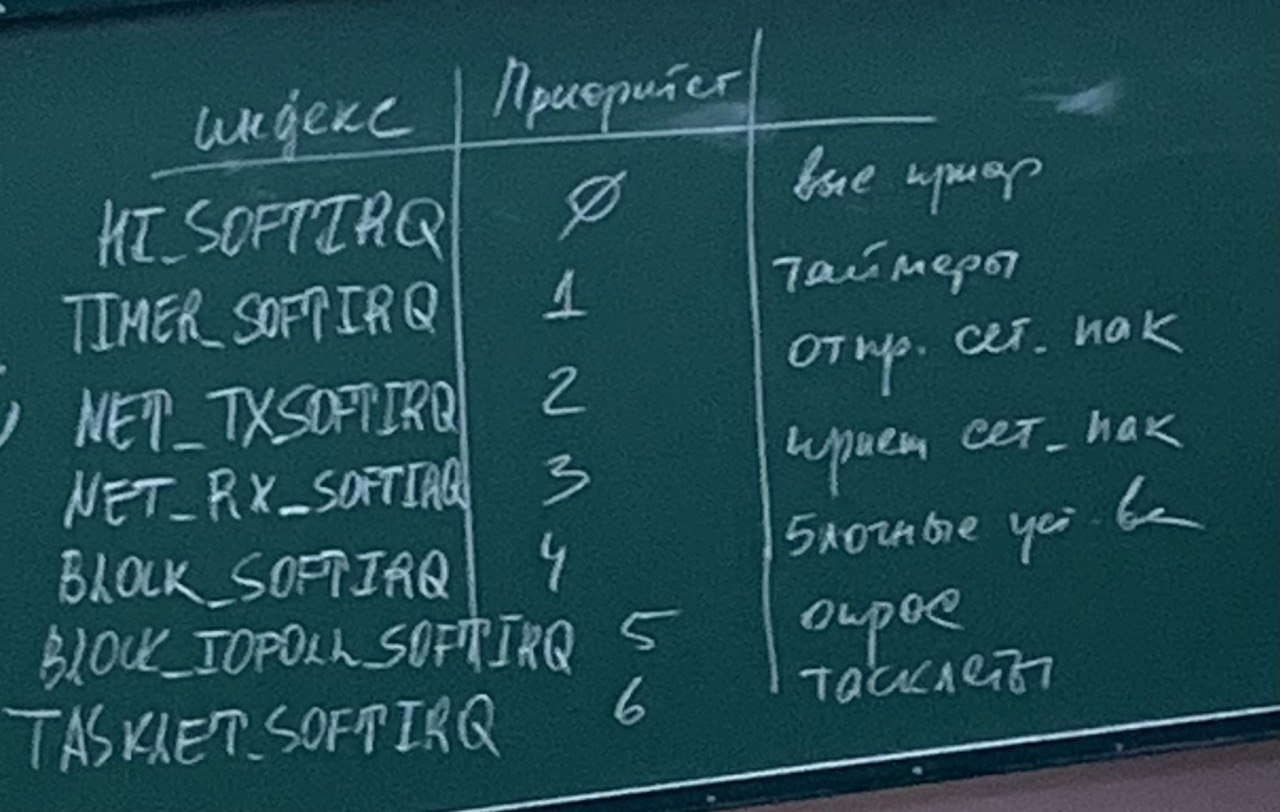
\includegraphics[scale=0.15]{pics/table_intr.jpg}}	\right{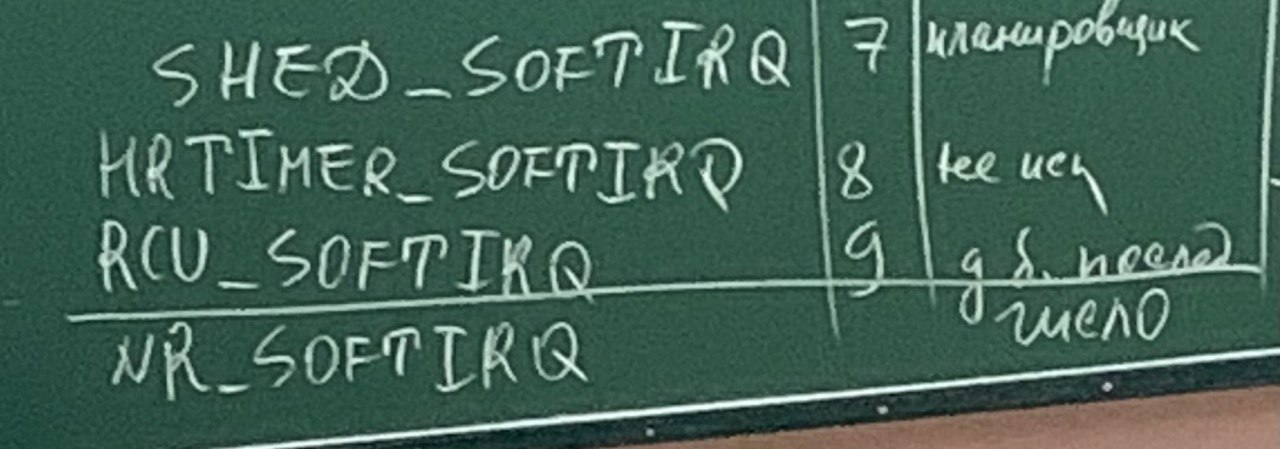
\includegraphics[scale=0.15]{pics/table_intr2.jpg}}
%\end{figure}

Основная задача сетевой системы - прием и отправка пакетов. Она не ограничивается одним пакетом.

\begin{lstlisting}
const char *const softirq_to_name[NR_SOFTIRQS] = {"HI", "TIMER", "NET_TX", "NET_RX", "BLOCK", "BLOCK_IO", "TASKLET", "SHED", "HRTIMER", "RCU"}.
\end{lstlisting}	

/proc/softirqs - здесь можно увидеть эту информацию, т.е. все перечисленные имена.

Определена функция, которая заполняет вектор softirq\_vec заданным типом softirq\_action:

\begin{lstlisting}
void open_softirq(int nr, void (*action)(struct softirq_action *))
{
	softirq_vec[nr].action = action;
}

void raise_softirq(unsigned int nr);
\end{lstlisting}

Для того, чтобы зарегистрированное отложенное прерывание было поставлено в очередь на выполнение, необходимо вызывать функцию raise\_softirq.

Добавить новый уровень softirq можно только путем перекомпиляции ядра. Т.е. число обработчиков softirq не может быть изменено динамически. При этом смысл имеет только новое softirq, имеющее индекс на 1 меньше индекса tasklet, т.к. нет смысла переопределять кол-во softirq, т.к. можно использовать тасклет.

Из перечисления видно, что тасклет является одним из типов softirq.

Функция raise\_softirq() с указанием конкретного индекса (softirq) д.б. вызвана из
ОАП, т.е. ОАП должен отметить конкретное softirq как то, которое должно быть поставлено
в очередь на выполнение.

Выполнение softirq. Проверка ожидающих выполнения обработчиков отложенных действий типа softirq вып. в следующих случаях:

\begin{enumerate}
	\item При возврате из аппаратного прерывания.
	\item В контексте потока ядра ksoftirqd.
	\item В любом коде ядра, в котором явно проверяются и запускаются ожидающие выполнения
	обработчики softirq (например, как это делается в сетевой подсистеме).
\end{enumerate}

Независимо от способа вызова softirq, его выполнение осуществляется функцией do\_softirq().
Эта функция ункция в цикле роверяет наличие отложенных прерываний, т.е. каждый поток ядра ksoftirqd выполняет функцию run\_ksoftirqd(), которая проверяет наличие отложенных действий типа softirq, и в зависимости от результата вызывает соотв. функцию.

\begin{figure}[!h]
	\center{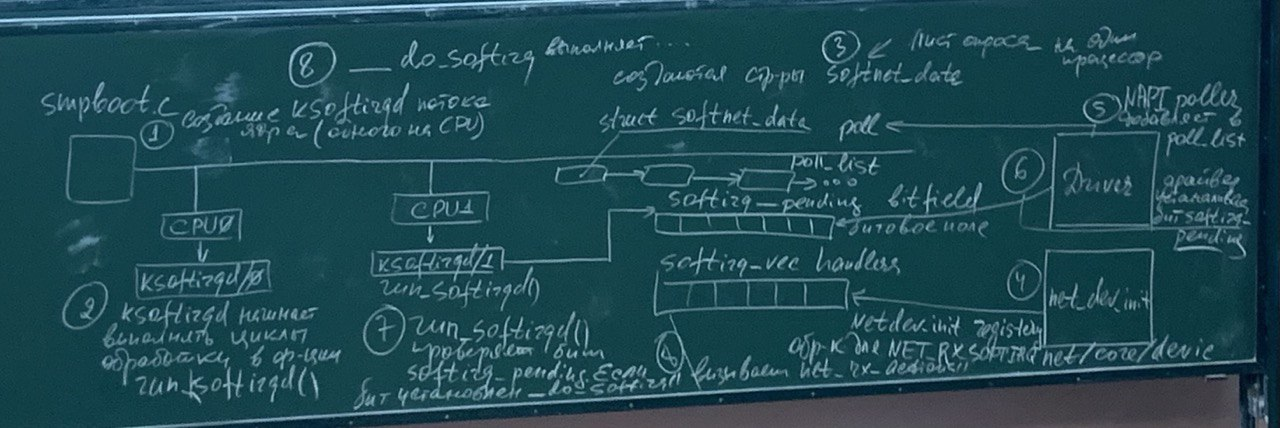
\includegraphics[scale=0.41]{pics/intr_schema.jpg}}
\end{figure}
	
\chapter{\textbf{Семинар 5 мая 2022}}

\section{Системный вызов open (продолжение)}

Лабораторная по \textbf{open} проводилась с целью демонстрации того, как работает ядро ОС. Ядро предоставляет приложениям интерфейс, который называется API (это системные вызовы). Приложение использует API, чтобы получить обслуживание запросов приложения, т.е. сервис.

Ни одна ОС не позволяет приложениям напрямую обращаться к внешним устройствам. Поле mode в [f]open обязателен, если установлен O\_CREATE, для этого файла нужно установить права доступа. Формируется битовая маска создания файла.

В struct file\_operations close отсуствтует, есть release.

\begin{lstlisting}[language=C]
SYSCALL_DEFINE3(open, const char __user *, filename, int, flags, umode_t, mode)
{
	if (force_o_largefile())
		flags |= O_LARGEFILE;
	return do_sys_open(AT_FDCWD, filename, flags, mode);
}	
	
long do_sys_open(int dfd, const char __user *filename, int flags, umode_t mode)
{
	struct open_how how = build_open_how(flags, mode);
	return do_sys_openat2(dfd, filename, &how);
}

struct nameidata {
	struct path	path;
	struct qstr	last;
	struct path	root;
	struct inode	*inode; /* path.dentry.d_inode */
	unsigned int	flags;
	unsigned	seq;
	int		last_type;
	unsigned	depth;
	char *saved_names[MAX_NESTED_LINKS + 1];
	
	/* Intent data */
	union {
		struct open_intent open;
	} intent;
};
\end{lstlisting}

\section{Разработка Virtual File System (VFS)}

В ядре Linux имеется структура file\_system\_type.

\begin{lstlisting}
struct file_system_type 
{
	const char *name;
	int fs_flags;
	#define FS_REQUIRES_DEV		1  
	...
	#define FS_USERNS_MOUNT		8	/* Can be mounted by userns root */
	struct dentry *(*mount)(struct file_system_type *,int,const char *, void *);
	void (*kill_sb) (struct super_block *);
	struct module *owner;
	struct file_system_type *next;
	...
};
\end{lstlisting}

ФС реализовывается в виде загружаемого модуля ядра. ФС становится доступной, если она подмонтирована. Функции суперблока выполняются при вызове mount, но описана также kill\_sb. В ядре имеется список таких структур (поле next). В системе может существовать только один тип ФС, например, ext2. В это же время одна и та же ФС может быть подмонтирована много раз, причем к разным директориям, которые будут для нее корневыми.

Рассмотрим пример объявления собственной ФС.

\begin{lstlisting}
struct file_system_type fuse_fs_type = 
{
	.owner = THIS_MODULE;
	.name = "fuse";
	.fs_flags = FS_HAS_SUBTYPE | FS_USERNS_MOUNT;
	.mount = fuse_mount;
	.kill_sb = fuse_kill_sb_anon;
}
\end{lstlisting}

Поле owner определяет кол-во ссылок на модуль. Он нужен для того, чтобы модуль не был выгружен, если ФС подмонтирована, т.к. это может привести к краху. Счетчик ссылок не 0 - выгрузить не удастся.

После объявления ФС, ее нужно зарегистрировать: register\_filesystem() в функции init, unregister\_filesystem() в функции exit.

Прежде чем мы сможем выполнить монтирование ФС, необходимо заполнить поля struct superblock и определить операции на суперблоке.

\begin{lstlisting}
static struct dentry *fuse_mount(struct file_system_type *fuse_fs_type, int flags, char const *dev, void *data)
{
	struct dentry *entry = mount_bdev(fuse_fs_type, flags, dev, data, fill_sb);
}
\end{lstlisting}

Нужно четко понимать, где мы регистрируем свою функцию, а где регистрируем функцию, описанную в ядре (generic).

\chapter{\textbf{Лекция 14 мая 2022}}

\section{Прерывания. Механизмы обслуживания прерываний в системе}

Простейшую схему получения процессором сигналов прерывания мы рассматривали ранее. В современных системах такая схема не удовлетворяет никаким потребностям, и информирование процессора о возникающих аппаратных прерываниях выполняется с помощью сигналов MSI (Message Signal Interrupt). Это серьезная поддержка аппаратной состовляющей системы, но мы не будем ее рассматривать.

В системе аппаратные прерывания делятся на быстрые и медленные с точки зрения их обсулживания в системе. Существует одно быстрое прерывание - от системного таймера. \textit{Быстрые перывания} имеют следующую особенность: их обработчики выполняются полностью, от начала до конца. \textit{Медленные прерывания} - все остальные, от внешних устройств, при этом в вычислительных системах все устройства - внешние. Такие обратчики реализуются в виде двух частей: верхняя и нижняя половина. Верхняя половина выполняется на высочайшем уровне приоритета. 

Когда выполняется обработчик АП в SMP-архитектуре, на том процессоре, на котором выполняется обработчик, запрещены все прерывания, а для других процессоров запрещены прерывания по этой линии IRQ. Обработчик АП должен завершаться как можно быстрее, поэтому он выполняет только самый необходимый объем действий, фактически его действия заключаются в получении данных с соотв. порта, к которому подключено внешнее устройство, и сохранение этих данных в буфере ядра. 

Кроме этого, обработчик АП должен инициализировать работу отложенного действия второй половины. Вторая пловина может быть реализована в виде softirq, tasklet или work queue. Каждый из перечисленных типов отложенных действий по обработке АП обладает особенностями, которые необходимо учитывать при выборе механизма реализации отложенных действий. 

Ранее рассмотрели softirq, которые определяются статически, в системе определено ограниченное количество softirq, при этом tasklet - вид softirq. Мы рассмотрели схему, которая демонстрирует как устроено отложенное действие для сетевой подсистемы компьютера, поскольку именно сетевая подсистема способна воспринимать большое количество приходящих пакетов, при этом возникают соотв. АП, их может быть большое количество, и это довольно объемная обработка, связанная с очередью соотв. сообщений. 

Демон ksoftirqd - поток ядра каждого процессора, задача которого - планирование и запуск на выполнение softirq. Когда машина нагружена гибкими прерываниями soft\_interrupts, которые обслуживаются при завершении АП, при этом таких прерываний в единицу времени может возникать много, каждое из этих АП инициализирует свой обработчик отложенного действия softirq, в результате в системе для каждого процессора создается очередь softirq, сюда же входят и tasklet. При этом, например, по размеру очереди или по времени работы ksoftirqd, можно определить степень давления на систему обращений от сетевого устройства. Сетевое устройство обращается к системе за обслуживанием. Это признак нагрузочной аттаки.

Чтобы управлять выполнением отложенных действий типа softirq, предназначены такие демоны.

\section{Tasklet-ы}

Tasklet - частный случай реализации softirq, но в отличие от softirq, которые пишутся таким образом, чтобы одновременно в системе могло выполняться некоторое количество одних и тех же softirq (в полном объеме реализовано взаимоисключение), на tasklet накладывается следующее ограничение: обработчик тасклета в каждый конкретный момент времени может выполняться только на одном процессоре, т.е. один и тот же тасклет не может выполняться параллельно, в отличие от softirq.

Поэтому в системах, в которых требуется быстрая реакция, предпочтение отдается softirq. Реализация тасклета намного проще, чем реализация softirq ввиду этого ограничения. Тасклеты - хороший компромисс между производительностью системы и простотой использования. 

В отличие от softirq, которые регистрируются при компиляции системы и их количество определено в системе, асклеты могут быть зарегистрированы как статически, так и динамически.

Тасклеты как объекты ядра описываются соотв. структурой.

\begin{lstlisting}[language=C]
struct tasklet_struct 
{
		struct tasklet_struct *next;
		unsigned long state;
		atomic_t count;
		bool use_callback;
		union 
		{
				void (*func)(unsigned long data);
				void (*callback)(struct tasklet_struct *t);
		};
		unsigned long data;
};

enum 
{
	TASKLET_STATE_SCHED, //Scheduled
	TASKLET_STATE_RUN // Running (executig)
}
\end{lstlisting}

В системе имеется связный список обработчиков тасклет. Поле state определяется по enum.

~

Таслет может быть объявлен статически или динамически:

\begin{lstlisting}[language=C]
\\Static
#include <linux/interrupts.h>

DECLARE_TASKLET(name, func, data);
DECLARE_TASKLET_DISABLED(name, func, data);

\\Dynamic
#define DECLARE_TASKLET(name, __callback)
struct tasklet_struct name = 
{
	.count = ATOMIC_INIT(0);
	.callback = __callback;
	.use_callback = true;
};

extern void tasklet_init(struct tasklet_struct *t,void (*func)(unsigned long), 
																												unsigned long data);

extern void __tasklet_schedule(struct tasklet_struct *t);

static inline void tasklet_schedule(struct tasklet_struct *t)
{
	if (!test_and_set_bit(TASKLET_STATE_SCHED, &t->state))
			__tasklet_schedule(t);
}

//High priority tasklet
extern void __tasklet_hischedule(struct tasklet_struct *t);

static inline void tasklet_hischedule(struct tasklet_struct *t)
{
	if (!test_and_set_bit(TASKLET_STATE_SCHED, &t->state))
			__tasklet_hischedule(t);
}

... tasklet_disable(...);
... tasklet_disable_nosync(...);
... tasklet_enable(...)

extern void tasklet_kill(struct tasklet_struct *t);
extern void tasklet_kill_immediate(struct tasklet_struct *t,unsigned int cpu);

void tasklet_handler(unsigned long data);

static inline tasklet_trylock(struct tasklet_struct *t)
{
	return !test_and_set_bit(TASKLET_STATE_RUN, &t->state);
}
\end{lstlisting}

Обработчик АП инцииализирует отложенное действие, чтобы его выполнить, необходимо запланировать тасклет.

Ограничение тасклета: тасклет не может блокироваться, т.е. в тасклетах нельзя использовать блокирующие примитивы. Если в тасклете используются общие с обработчиком прерывания или каким-то другим тасклетом данные, то необходимо использовать спинлоки. 

Свойства тасклетов:

\begin{itemize}
	\item Если вызывается функция tasklet\_schedule(), то тасклет гарантировано будет выполняться на каком-то процессоре, хотя бы один раз после этого. 
	\item Если тасклет уже запланирован, но его выполнение еще не началось, то он обязательно будет один раз выполнен через какое-то время. 
	\item Если тасклет уже выполняется на другом процессоре или планирование тасклета вызвано из самого кода тасклета, то его перепланирование будет отложено.
	\item Если один и от же тасклет выполняется несколько раз (он может даже сам себя запланировать), то для монопольного доступа к разделяемым данным необходимо использовать спинлоки.
	\item В системе имеется определенная на тасклетах функция блокировки: tasklet\_trylock().
\end{itemize}

\section{Workqeue (Очереди работ)}

Очереди работ, в отличие от тасклетов, могут блокироваться, но между ними значительно больше отличий. Главное отличие - гибкими прерываниями, тасклетами <<руководит>> ksoftirqd, а очереди работ в системе реализованы совершенно по-другому.

Наибольшие изменения произошли с очередями работ в связи с управлением параллельным выполнением очередей работ, и это связано с SMP-архитектурой.

Несколько концепций очередей работ workqueue представляют собой связанные с работой структуры данных, которые легко перепутать, т.е. в ядре в отличие от тасклетов, над которыми определена одна структура, над очередями определено несколько структур, каждая из которых играет важную роль. 

Работа - та работа, которую должен выполнить обработчик отложенного действия. работы ставятся в некоторую очередь, при этом в одну очередь работ может быть поставлено много работ. Работа связывается с конкретной очередью. В системе определен т.н. worker (рабочий) - поток ядра (work thread). В системе имеется worker pull - множество worker, один worker может принадлежать одному pull.

Посредник, ответственный за установку отношений между workqueue и worker pull(?).

Существенные \textbf{отличия} между тасклетами и очередями работ:

\begin{enumerate}
	\item Тасклеты выполянются в констексте прерывания, в результате чего код тасклета должен быть неделимым(atomic). В отличие от тасклетов, workqueue выполняются в контексте специальных потоков ядра, и как результат имеют большую свободу действий, и в частности очереди работ могут блокироваться или засыпать.
	\item Тасклеты всегда выполняются на процессоре, на котором выполнялось АП, запланировавшее данный тасклет. Очереди по умолчанию также выполняются на том же процесосоре, но могут выполняться и на других процессорах.
	\item Код ядра требует, чтобы выполнение функций очередей работ откладывалось на
	определенный интервал времени.
	\item Ключевое отличие - тасклеты выполняются за короткий период времени после того, как были запланированы, а очереди работ имеют значительно большие задержки и необязательно должны быть атомарными, неделимыми.
\end{enumerate}

Каждый из перечисленных механизмов обладает существенными отличиями, поэтому выбор соотв. механизма должен быть осмысленным и обоснованным.

\begin{lstlisting}[language=C]
	//linux 3.18.22
	struct workqueue_struct
	{
		struct list_head pwqs;
		struct list_head list;
		struct mutex mutex;
		...
		char name[WQ_NAME_LEN];
		struct rcu_head rcu;
		...
	};
	
	struct work_struct 
	{
		atomic_long_t data;
		struct list_head entry;
		work_func_t func;
		#ifndef CONFIG_LOCKDEP
		struct lockdep_map lockdep_map;
		#ednif
	};
\end{lstlisting}

List\_head - список всех очередей работ, но на конкретное CPU существует свой список rcu\_head, чтобы не перебирать все очереди работ.

Так же как для тасклетов, работу (задачу как отложенное действие) можно поместить в очередь работ как статически, так и динамически. 

\begin{lstlisting}[language=C]
//static
DECLARE_WORK(name, void (*func)(void*)); //name = work_struct instance

//dynamic
#ifndef CONFIG_LOCKDEP
#define __INIT__WORK(__work, __func, __onstack)
	do 
	{
			static stuct lock_class_key __key;
			__init_work((__work), __onstack);
			(__work)->data = (atomic_long_t)WORK_DATA_INIT();
			INIT_LIST_HEAD(&(__work)->entry);
			(__work)->func = (__func);
	}
	while(0);

#define INIT_WORK(__work, __func)
	__INIT_WORK((__work), (__func), 0)
	
typedef void (*work_func_t)(struct work_struct *work);

PREPARE_WORK();

int alloc_workqueue(char *name, unsigned int flags, int max_active);

//Flags
enum {
	WQ_UNBOUND = 1 << 1;
	WQ_FREZABLE = 1 << 2;
}
\end{lstlisting}

Если имеется хоть какая-то возможность, что структура уже инициализирована, лучше вместо init\_work() использовать prepare\_work().

Для создания очереди работ, до 2.6.36, использоваласть create\_workqueue(), в более современных версиях - alloc\_workqueue(). Flags определяет как очередь работ будет выполняться, max\_active - ограничивает число задач, которые одновременно будут стоять в чоереди к cpu.

\chapter{\textbf{Семинар 19 мая 2022}}

\section{Сокеты}

Сокеты - универсальное средство взаимодействия параллельных процессов. Нужно сравнивать со средствами взаимодействия из systemfive. 

Универсальность заключается в том, что сокеты используются как и на локальной машине, так и в распределенной системе (сети), в отличие от, например, разделяемой памяти, которая применима только на отдельно стоящей машине.

Различают 3 типа сокетов:

\begin{itemize}
	\item Парные - альтернатива pipe, но в отличие от них обеспечивают дуплексную связь;
	\item Сокеты домена UNIX - предназначены для взаимодействия параллельных процессов на локальной машине по модели клиент-сервер;
	\item Сетевые (af net) сокеты - предназначены для взаимодействия параллельных процессов в распределенной сети по модели клиент-сервер.
\end{itemize}

Сокет - абстракция конечной точки взаимодействия, потому что для разных систем сокет поддерживается в системе разными средствами. Система предоставляет пользователю соответствующее API. 

\begin{lstlisting}
int socket(int family, int type, int protocol);
\end{lstlisting}

\begin{figure}[!h]
	\center{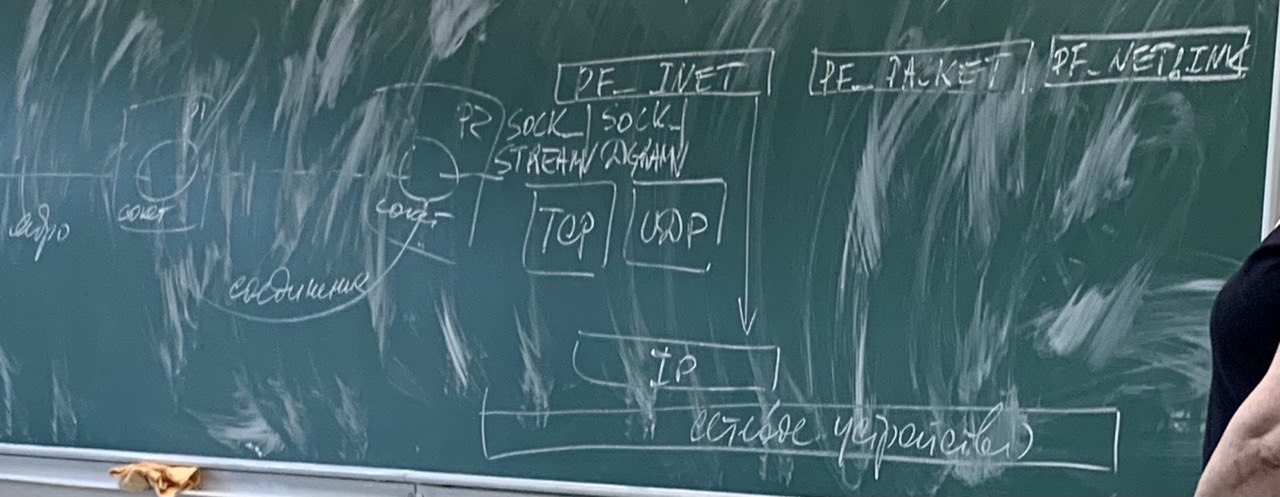
\includegraphics[scale=0.41]{pics/socket.jpg}}
\end{figure}

Здесь показаны сокеты в UNIX BSD. Самым важным моментом здесь является SOCK\_STREAM TCP и SOCK\_DEGRAM UDP. 

PF\_PACKET - сокеты для профессиональной деятельности, созданные для непосредственного доступа приложения к сетевым устройствам. 

PF\_NETLINK - группа сокетов, созданных для обмена информацией между частями ядра, еще один интерфейс ядра, которая позволяет получить информацию из ядра в пользовательское пространство.

Функция socket в результате приведет к вызову sys\_socket, но в Linux имеется один единственный вызов и он работает как switch.

\begin{lstlisting}
asmlinkage long sys_socketcall(int call, unsigned long *args)
{
	unsigned long a[6];
	unsigned long a0,a1;
	int err;
	
	if(call < 1 || call > SYS_RECVMSG)
		return -EINVAL;
	
	/* copy_from_user should be SMP safe. */
	if (copy_from_user(a, args, nargs[call]))
		return -EFAULT;
	
	a0=a[0];
	a1=a[1];
	
	switch(call) 
	{
		case SYS_SOCKET: err = sys_socket(a0,a1,a[2]); break;
		case SYS_BIND: err = sys_bind(a0,(struct sockaddr *)a1, a[2]); break;
		case SYS_CONNECT: err = sys_connect(a0, (struct sockaddr *)a1, a[2]);
		.....
		default: err = -EINVAL; break;
	}
	return err;
}
\end{lstlisting}

В switch перечисляются все функции, определенные на сокетах. Каждая из функций реализуется в ядре. Например:

\begin{lstlisting}
asmlinkage long sys_socket(int family, int type, int protocol)
{
	int retval;
	struct socket *sock;
	
	retval = sock_create(family, type, protocol, &sock);
	if (retval < 0)
		goto out;
	
	retval = sock_map_fd(sock);
	if (retval < 0)
		goto out_release;
	
	out:
	/* It may be already another descriptor 8) Not kernel problem. */
	return retval;
	
	out_release:
	sock_release(sock);
	return retval;
}
\end{lstlisting}

Функция sock\_create() инициализирует поля структуры socket. Рассмотрим эту структуру.

\begin{lstlisting}
struct socket 
{
	socket_state            state;
	short                   type;
	unsigned long           flags;
	struct socket_wq __rcu  *wq;
	struct file       			*file;
	struct sock             *sk;
	const struct proto_ops  *ops;
}
\end{lstlisting}

У сокета различают 5 состояний, 4 из которых - стадии соединения:

\begin{itemize}
	\item SS\_FREE - свободный сокет, с которым можно соединяться;
	\item SS\_UNCONNECTED - несоединенный сокет;
	\item SS\_CONNECTING - сокет находится в состоянии соединения;
	\item SS\_CONNECTED - соединенный сокет;
	\item SS\_DISCONNECTING - сокет разъединяется в данный момент.
\end{itemize}

Флаги используются для синхронизации доступа к сокетам. 

Важнейшим полем является структура proto\_ops (от слов protocol operations). Операции на сокетах зависят от типа сокета, но протокол зависит от типа сокета.

Первым параметром является family (или domain). AF = address family, можно перевести как пространство имен.

\begin{itemize}
	\item AF\_UNIX - эти сокеты предназначены для межпроцессорного взаимодействия на локальном компьютере;
	\item AF\_INET - эти сокеты предназначены для взаимодействия параллельных процессов в распределенных системах, а именно в интернете версии 4, т.е. доменом является любая ipv4-сеть, также это сокеты семейства протоколов tcp/ip;
	\item AF\_INET6 - ipv6;
	\item AF\_IPX - семейство протоколов ipx;
	\item AF\_UNSPEC - неопределенный домен.
\end{itemize}

Поле type содержит тип сокета. Это второй параметр в функции socket. Он может иметь значение:

\begin{itemize}
	\item SOCK\_STREAM - сокеты потоков, они определяют ориентированное на потоки надежное упорядоченное полнодуплексное логическое соединение между двумя сокетами(point to point);
	\item SOCK\_DEGRAM - определяют ненадежную службу DATAGRAM без установления логического соединения, причем пакеты могут передаваться без сохранения порядка (т.н. широковещательная передача данных). Альтернатива - 1-ый тип;
	\item SOCK\_RAW - низкоуровневый интерфейс DATAGRAM по протоколу IP, причем необязательно posix1, сокет взаимодействует с сетевым устройством напрямую;
	\item SOCK\_RDM;
	\item SOCK\_SEGPACKET;
	\item SOCK\_PACKET - не используется.
\end{itemize}

Основными типами сокетов являются SOCK\_STREAM, SOCK\_DEGRAM, SOCK\_RAW.

Третий параметр - протокол. Протоколы выбираются в зависимости от семейства и типа сокета. Обычно этот параметр имеет значение 0, в этом случае протокол выбирается по умолчанию. 

Для протоколов также устанавливаются обозначения. Это IPPROTO\_*, например IPPROTO\_TCP, IPPROTO\_DEGRAM, IPPROTO\_UTP.

Для семейства AF\_INET для типа сокета SOCK\_STREAM всегда будет выбираться IPPROTO\_TCP.

Для семейства AF\_INET для типа сокета SOCK\_DEGRAM всегда будет выбираться IPPROTO\_UTP.

Посколько сокеты - абстракция конечных точек соединения, то необходимо указать адреса этих точек соединения. Поэтому в системе определена структура sockadrr. Она определена в общем виде, потому что существуют разные типы, семейства и протоколы сокетов.

\begin{lstlisting}
struct sockaddr 
{ 
	unsigned short  sa_family; // Address family, i.e. AF_xxx 
	char 			sa_data[14]; // 14 bytes for adress storing
};
\end{lstlisting}

Сокеты в файловом пространстве имен: сокеты семейства AF\_UNIX. После создания такого сокета его можно увидеть в ФС командой ls как специальный файл, обозначаемый буквой s. 

Сетевые сокеты мы здесь не увидим. Сетевые сокеты мы можем увидеть только с помощью специальных команд, посмотрев номер соответствующего порта.

Рассмотрим фрагмент программы для сокетов семейства AF\_UNIX, демонстрирующий каким образом для этих сокетов заполняются поля структуры sockaddr.

\begin{lstlisting}
sock = socket(AF_UNIX, SOCK_DGRAM, 0);
if (sock < 0) 
{
	perror("socket failed");
	return EXIT_FAILURE;
}
srvr_name.sa_family = AF_UNIX;
strcpy(srvr_name.sa_data, "socket.soc");
if (bind(sock, &srvr_name, strlen(srvr_name.sa_data) + 
													sizeof(srvr_name.sa_family)) < 0) 
{
	perror("bind failed");
	return EXIT_FAILURE;
}
\end{lstlisting}

Здесь мы видим, что установлено семейство AF\_UNIX и тип SOCK\_DGRAM. Если использовать другой тип, ошибки не будет, но в этом не будет смысла, потому что, как мы видим, у нас как раз второй параметр (sa\_data) определяет имя специального файла, и взаимодействие сокетов AF\_UNIX выполняется через файловую подсистему (через специальные файлы), поэтому никакой потери данных не будет.

Для UNIX для сокетов AF\_INET такой общий адрес struct sockaddr не подходит. Для взаимодействия процессов в сети необходимо указывать адреса и номер порта, поэтому структура не подходит. Поэтому для интернета была определена другая структура:

\begin{lstlisting}
struct sockaddr_in
{ 
	short int sin_family; // AF_NET
	unsigned short int sin_port; // Port number
	struct in_addr sin_addr; // IP-adress
	unsigned char sin_zero[8]; // Offsetting to the size of struct sockaddr
};
\end{lstlisting}

\begin{lstlisting}
struct in_addr {
	unsigned long s_addr;
};
\end{lstlisting}

Порядок байтов: little (аппаратный) endian и big (сетевой) endian. Поскольку речь идет о значениях адресов, то этот порядок имеет значение. Чтобы не возникало неоднозначности при получении адресов, используются 4 функции. 

\begin{lstlisting}
uint16_t htons(uint16_t hostint16);
uint32_t htonl(uint32_t hostint32);

uint16_t ntohs(uint16_t hostint16);
uint32_t ntohl(uint32_t hostint32);
\end{lstlisting}

Эти функции надо использовать всегда. Если сетевой и аппаратный порядок байтов совпадают, то эти функции не будут выполняться.

\chapter{\textbf{Лекция 28 мая 2022}}

\section{Прерывания. Механизмы обслуживания прерываний в системе. Очереди работ.}

Ранее перечислили объекты, которые определены в системе для работы с очередями работ: work, workqueue, worker, worker pull, pwq (pull worker queue).

Флаги (на прошлой лекции еще 2 флага было):

\begin{lstlisting}[language=C]
WQ_MEM_RECLAIM
WQ_HIGHPRI
WQ_SYSFS
WQ_MAX_ACTIVE
\end{lstlisting}

Очереди высокого приоритета (WQ\_HIGHPRI) выполняются в первую очередь. Есть очереди нормального приоритета.

Флаг WQ\_MAX\_ACTIVE имеет смысл только для привязанных очередей. С этим флагом очереди могут потреблять большое кол-во процессорного времени.

В соответствии с этим флагом (см. прошлую лекцию) очереди делятся на привязанные (normal) и непривязанные (unbound). Для нормальных очередей характерно то, что они выполняются на том же ядре, на котором выполнялось аппаратное прерывание, также как и тасклет. Это полезно для системы, т.к. в этом случае более оптимально использование кэша, но с другой стороны привязанные очереди повышают энергопотребление.

Флаг FREEZABLE: свойство очередей, их важное отличие от тасклетов, они могут переходить в состояние блокировки. Если в тасклете реализуется доступ к критическим секциям, там могут использоваться только спинлоки, а очереди работ могут блокироваться.

Для того, чтобы свести воедино все перечисленные объекты, рассмотрим следующую схему.

На каждое ядро имеется 2 типа workerpool: нормального (normal) и высокого (high) приоритета.

\begin{figure}[!h]
	\center{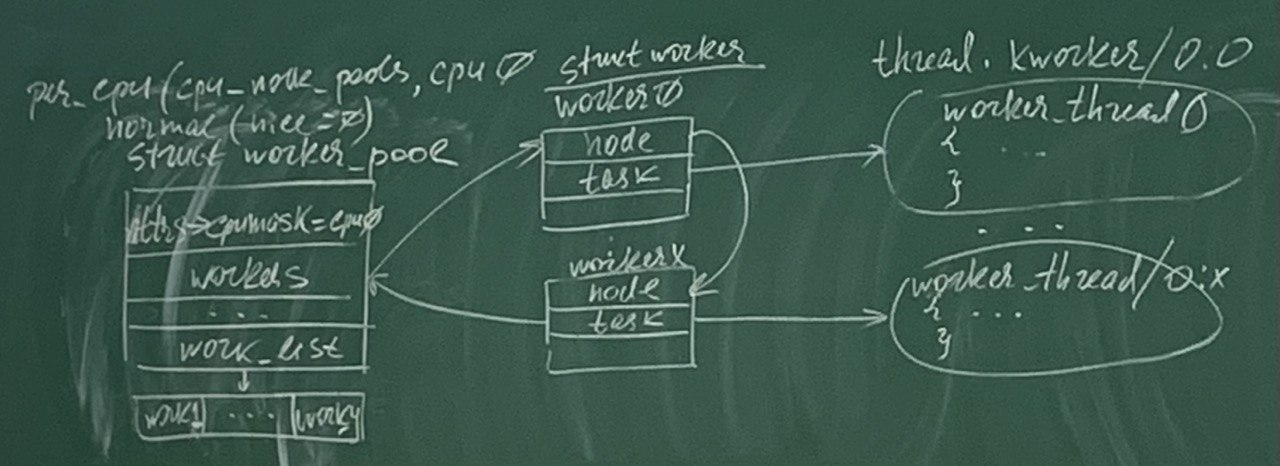
\includegraphics[scale=0.4]{pics/work1.jpg}}
\end{figure}

\begin{figure}[!h]
	\center{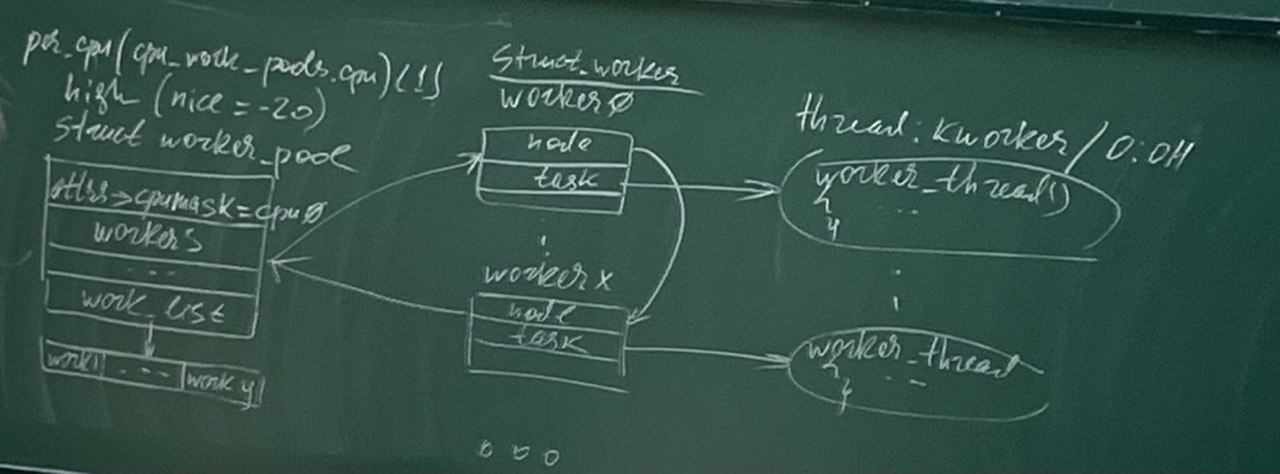
\includegraphics[scale=0.4]{pics/work2.jpg}}
\end{figure}

Ставим многоточие для каждого процессора на схеме.

Если ставится задача обработки информации в ядре, то ядро предоставляет механизм очередей работ, при этом в современных ПК это потоки ядра. В структуре есть поле task, речь идет о thread. Это особенность UNIX/Linux: не различаются процессы и потоки. В ядре есть функция clone(), по современным представлениям у нас многопоточное программирование, но UNIX изначально писался для паралелльного программирования. Мы это прорабатывали, используя fork() и create\_thread(). 

Для процесса, созданного с помощью fork, характерно все то, что характерно процессу. Именно поэтому казывается, что в Linux существует task\_struct, будь то процесс или поток. Разница может заключаться в том, что потоки могут не все наследовать, для этого надо указывать соотв. флаги. Нет смысла наследовать все для потока от процесса.

\section{5 моделей ввода-вывода}

\subsection*{Блокирующий ввод-вывод (синхронный)}

Это то, что мы изучали ранее все время. Асинхронный ввод-вывод невозможен для обычных файлов, т.е. на обычных файлов реализовывать соотв. флаги нельзя, т.е. при работе с обычными файлами всегда будут блокировки. 

Блокровки - зло, они занимают время, причем это время нельзя предсказать, они случайные, и проблема очевидная: если не блокироваться, то может возникнуть ситуация, как здесь нарисовано - datagram not ready (данные не готовы) - и тогда что мы считаем? В этом случае системный вызов должен вернуть ошибку, а процесс должен сноза запросить данные. Здесь это невозможно.  Не рекомендуется делать блокировки там, где это не необходимо. 

Также приведена картинка из книги Шоу - Логическое проектирование ОС. Древняя диаграмма, он она очень полезная, показывающая, что когда приложение запрашивает ввод/вывод, оно блокируется.

\begin{figure}[!h]
	\center{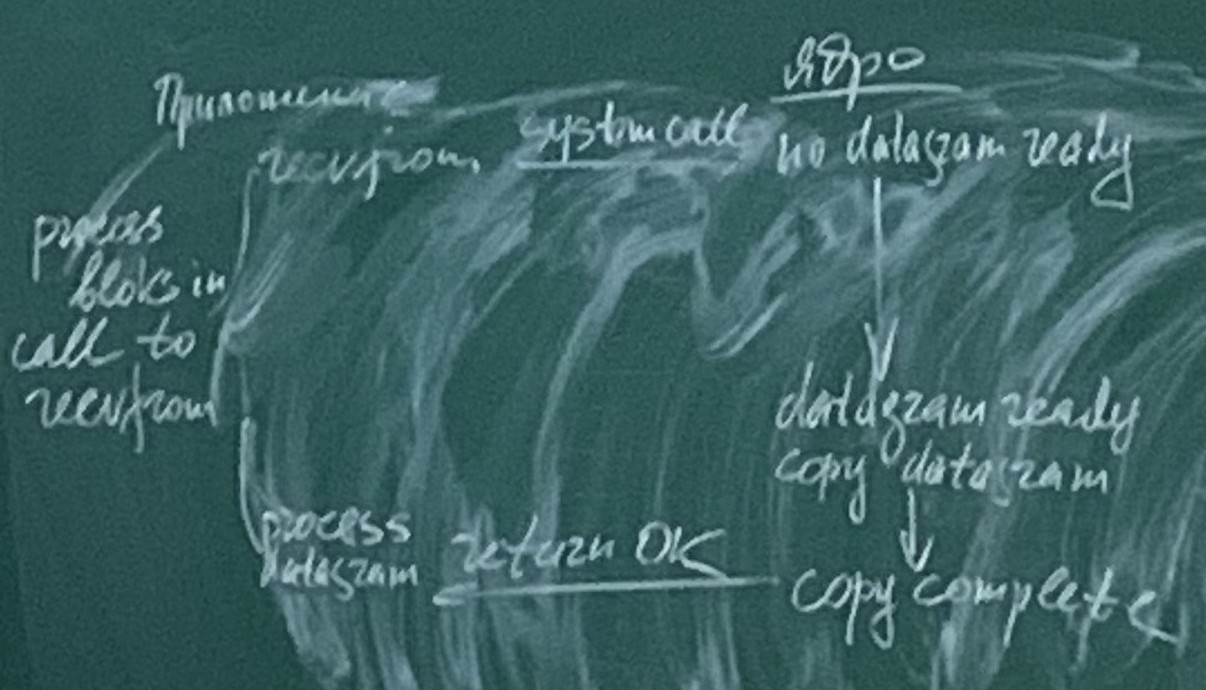
\includegraphics[scale=0.3]{pics/work3.jpg}}
\end{figure}

\begin{figure}[!h]
	\center{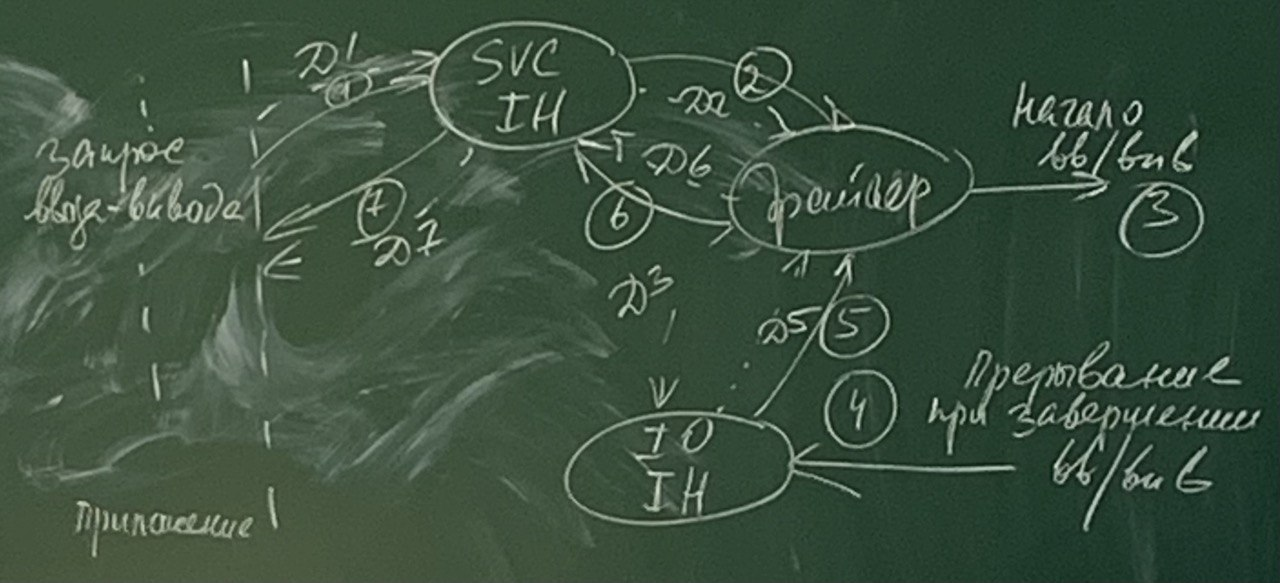
\includegraphics[scale=0.4]{pics/work4.jpg}}
\end{figure}

Процессор не управляет операцией ввода-вывода, он выключается переходит на выполнение другой работы именно в рамках архитектуры, в которой реализовано распараллеливание функций. Соответственно, запросив ввод-вывод, приложение блокируется и оно пробуждается, когда внешнее устрйоство завершает операцию ввода-вывода, формирует сигнал прерывания, который приходит на контроллер прерывания и этот сигнал с контроллера прерывания в самой простейшей схемы поступает на выделенную ножку процессора в конце выполнения каждой команды процессор проверяет наличия сигнала прерывания на этой ножке, если он пришел - процессор переходит на обработку, для этого он должен адресовать прерывание, для этого в системе есть IDT.

Даже если при выполнении операции ввода-вывода не удалось прочитать или записать данные, все равно приложение получит сообщение об ошибке. В любом случае приложение получит некоторую информацию.

\subsection*{Неблокирующий ввод-вывод (pooling, опрос)}

Везде используем recfrom(), а не read/write, это показатель того, что речь идет не об обычных файлах, например может идти о пайпах, передаче сообщений, о сокетах.

\begin{figure}[!h]
	\center{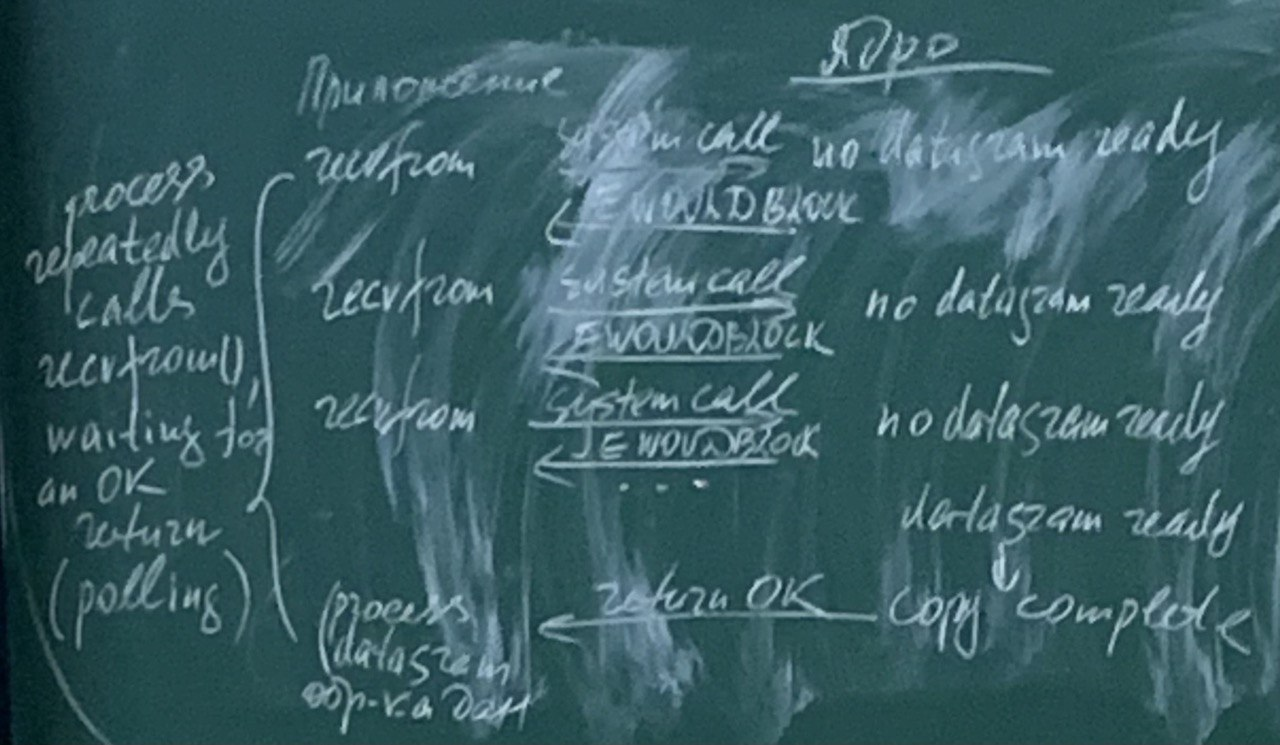
\includegraphics[scale=0.4]{pics/work5.jpg}}
\end{figure}

В данном случае мы видим, что процесс не блокируется, но постоянно запрашивает данные. Получив ошибку, что данные не готовы, он опять выполняет запрос. Это крайне затратная схема. Процессор контроллирует процесс ввода-вывода, постоянно опрашивая готовность внешнего устройства, соотв. готовность устанавливается устройством с помощью флагов, т.е. процессор постоянно опрашивает флаги готовности внешнего устройства. 

Когда устройство готово, данные аппаратаным прерыванием будут записаны в буфер ядра, а потом каким-то отложенным действием они будут в дальнейшем дообработаны и доведены до приложения. 

Этот опрос - самая первая схема, которая была реализована в вычислительных машинах. Прерывания полноценно появились лишь в 3 поколении ЭВМ, когда была реализована идея распараллеливания функций. Раз процессор отключается от управления внешним устройством, его нужно проинформировать, что операция ввода-вывода завершена.

Для этой модели характерны большие накладные расходы.

\subsection*{Мультиплексирование ввода-вывода}

При реализации этой модели используется один из мультиплексеров: select, pselect, poll, epoll.

Пишут, что select неэффективен, pselect практически как select, более эффективным мультиплексором является poll и его более современная версия epoll. 

Мультиплексер (коммутатор) - устройство, которое объединяет информацию, поступающую по нескольким каналам ввода, и выдает ее по одному выходному каналу. Процесс совмещения нескольких сообщений, передаваемых одновременно, в одной физической или логической среде. 

Существует 2 основных вида мультиплексирования: временнОе и частотное. 

\begin{figure}[!h]
	\center{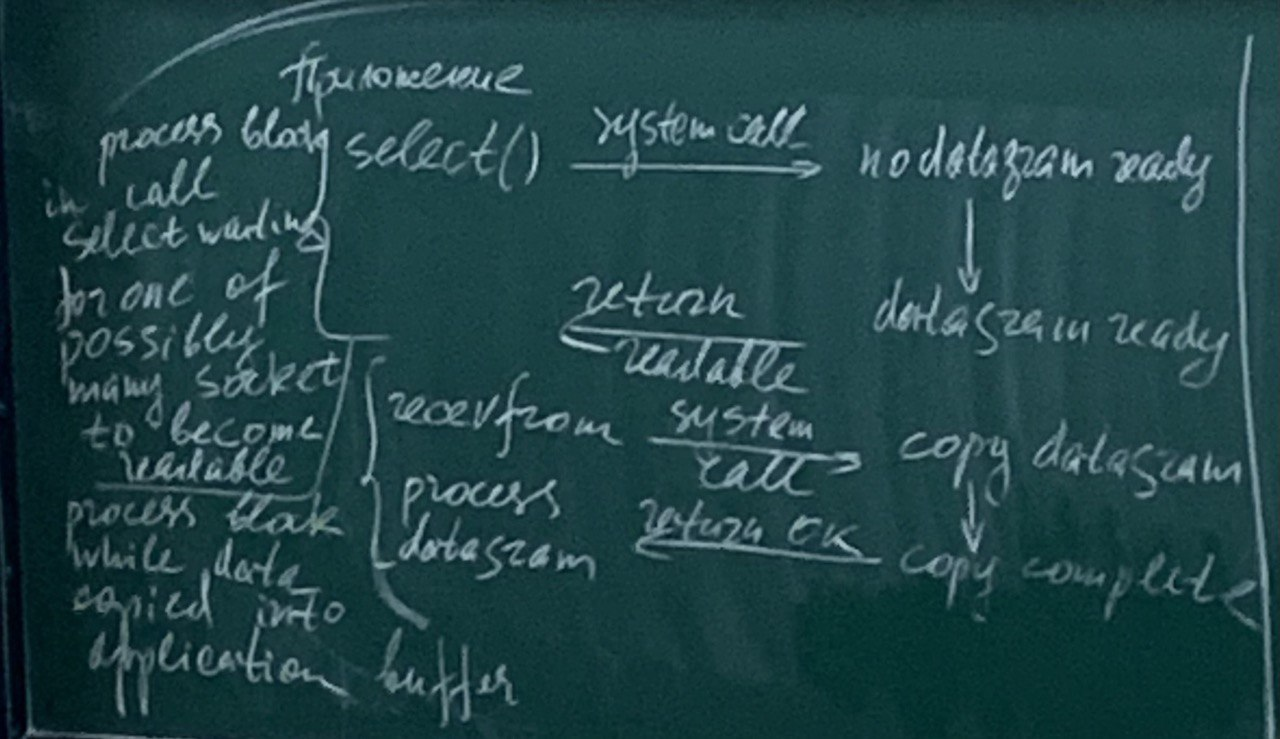
\includegraphics[scale=0.38]{pics/work6.jpg}}
\end{figure}

\begin{figure}[!h]
	\center{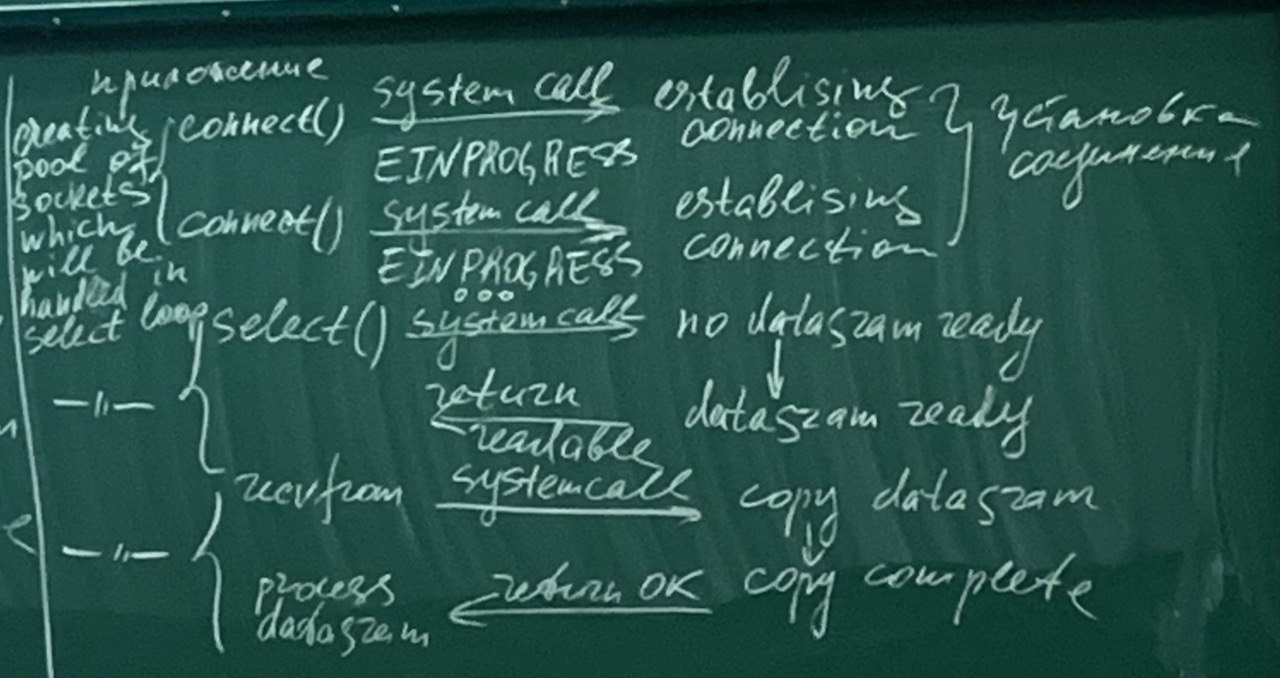
\includegraphics[scale=0.39]{pics/work7.jpg}}
\end{figure}

Более подробная диаграмма позволяет получить более детальную информацию о том, что происходит.

Приложение-клиент обращается к сокету, для этого вызывает системный вызов connect, чтобы установить связь с приложением-сервером. Здесь сеодинены запросы клиентов и работа на стороне сервера. Системный вызов select или poll выполняется на стороне сервера, клиенты устанавливают соединение.

Смысл мультплексирования: на мультиплексере все равно происходит блокировка, но на вопрос, какая блокировка будет занимтаь меньше времени: блокировка, где сокеты опрашиваются строго по порядку, или когда с помощью соотв. переключателя опрашивается весь пул сокетов и начинает обрабатываться сразу первый готовый сокет. 

Ведь возможна такая ситуация, когда 1 и 2 сокет не готовы, а 3 готов, но система будет блокирована на 1 сокете, ожидая его готовность. В это время можно было бы начать обрабатывать информацию от другого сокета, для этого надо использовать мультиплексера.

Блокировка с использованием мультиплексера будет занимать меньше времени. Т.е. при мультиплексирование будет обрабатывать первый готовый сокет.

Вариантом релазиции такого подхода является многопоточность, но следует иметь в виду, что в Linux очень <<дорогие>> потоки, потому что при создании UNIX была создана система, в которой реализавана иде fork, создания дочерних процессов, которая оказалась крайне эффективной, и вроде как потоки не внесли новые рассуждения. В UNIX ничего не стоит создать параллельные процессы. Игра идет на флагах, которые устанавливают уровень наследованя. 

Python: GIL (Global Interpreter Lock), в каждом процессе может выполняться только один поток. Это связано с тем, что в питоне используется GIL - глобальная блокировка, которая накладывает ограничения на потоки, т.е. нельзя одновременно использовать несколько процессов.

\subsection*{Ввод-вывод, управляемый сигналами (signal-driven IO)}

\begin{figure}[!h]
	\center{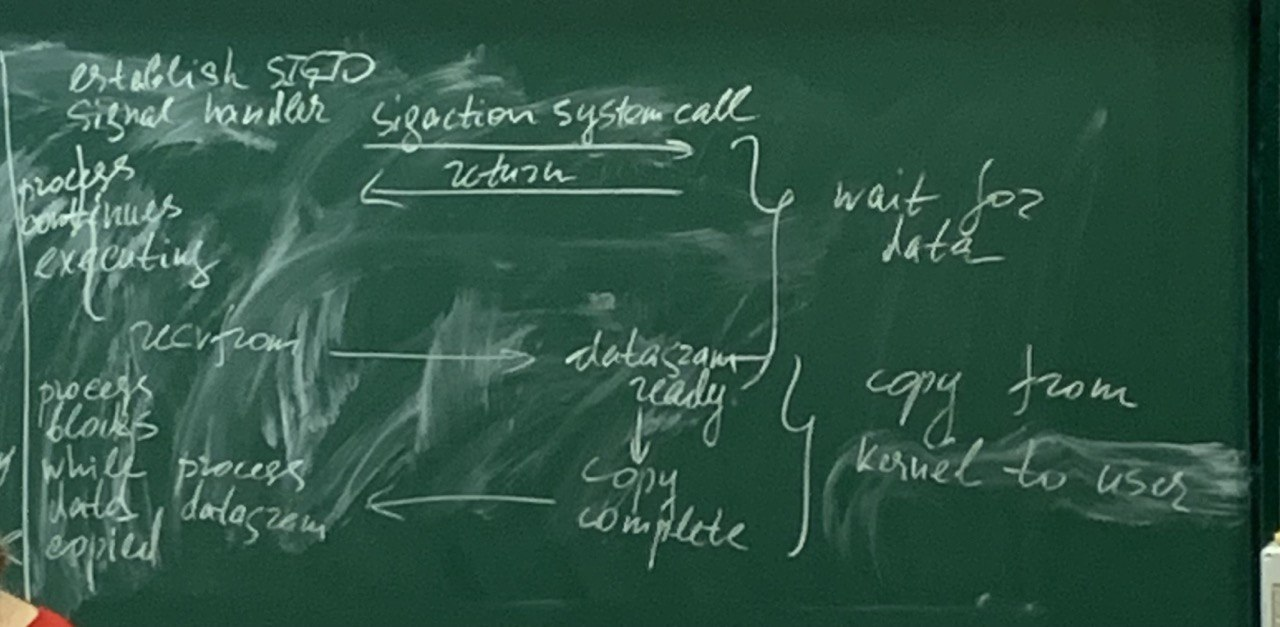
\includegraphics[scale=0.4]{pics/work8.jpg}}
\end{figure}

Сигнал SIG\_IO должен быть определен в системе, соотв. функция sigaction может установить собственный обработчик этого сигнала или можно использовать обработчик по умолчанию. 

Это уже асинхронный ввод-вывод, и процесс продолжает выполняться. Он блокируется только для того, чтобы дождаться получения данных. 

Для того, чтобы реализовать такой асинхронный ввод-вывод, ядро должно взять на себя всю работу, у сигнала SIG\_UO есть обработчик, который ждет возникнования сигнала, работу по посылке этого сигнала выполняет ядро, которое отслеживает готовность данных. Когда данные готовы, ядро пошлет сигнал SIG\_IO, в результате будет вызван обработчик этого сигнала, при этом функцию recfrom можно вызывать либо в обработчике сигнала, либо в основном потоке приложения.

Сигнал типа SIG\_IO для каждого процесса может быть только один. В результате, используя сигнал SIG\_IO, можно работать только с одним файловым дескриптором.

\subsection*{Асинхронный ввод-вывод, использующий специальные команды, которые называются }

Для такого ввода-вывода используются специальные команды, которые называются aio\_read, aio\_write, и тд.

\begin{figure}[!h]
	\center{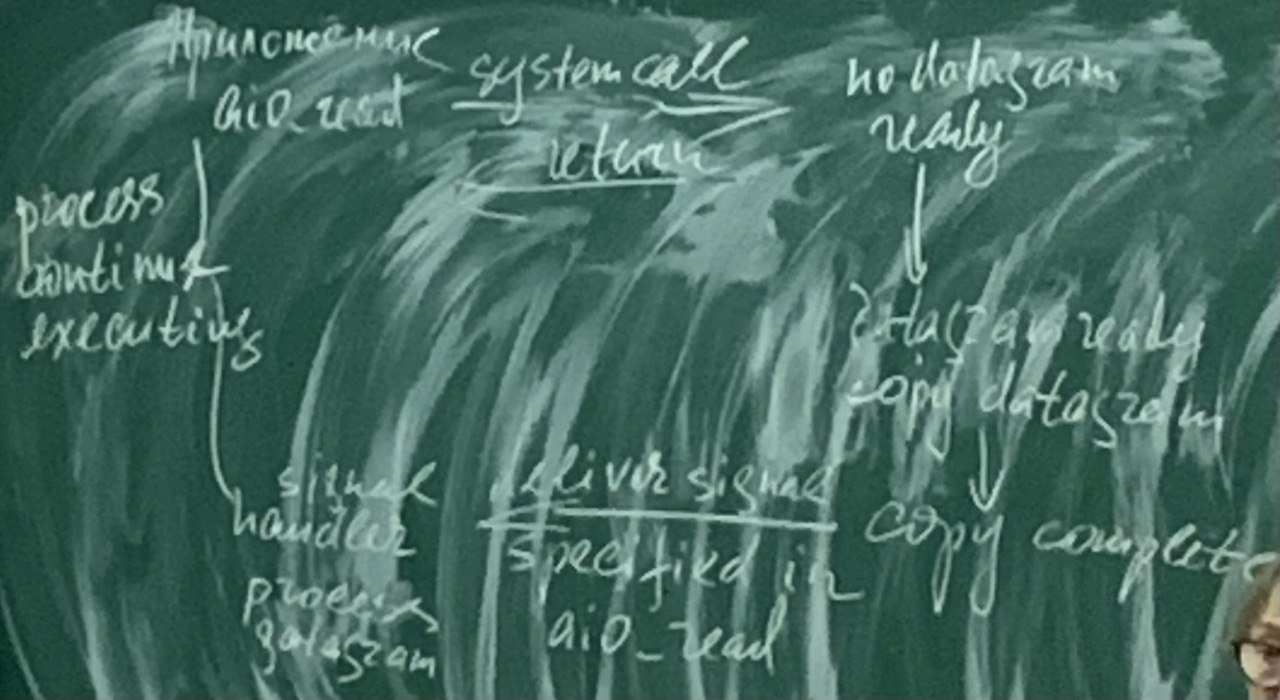
\includegraphics[scale=0.4]{pics/work9.jpg}}
\end{figure}

Проблема асинхронного ввода: определить, что может делать приложение, не получив данные? Время выполнения действий соотв. приложением будет меньше, т.е. отзывчивость такой системы может быть меньше при правильном написании.

\chapter{\textbf{Семинар 2 июня 2022}}

\section{Сокеты в файловом пространстве имен}

Название темы подчеркивает особенности этих сокетов. Именно такие сокеты мы можем увидеть в файловой подсистеме.

Что значит увидеть сокет в файловой подсистеме? С помощью команды ls -ial, увидим, что у него и inode есть, он помечен как специальный файл(s). Механизм передачи - \textit{скорее всего} буфер, который определен в файловой подсистеме. Второй тип сокетов - AF\_INET (сетевые). 

Все сокеты (AF\_UNIX, AF\_INET) взаимодействуют по модели клиент-сервер: это означает, что есть сервер, по своему названию это сервис, т.е. он предоставляет обслуживание, а клиенты запрашивают это обслуживание, передавая серверу запросы в сообщениях, т.е. взаимодействие клиент-сервер предполагает как получение сообщений сервером от клиентов, так и посылка сервером ответов клиентам. 

\begin{figure}[!h]
	\center{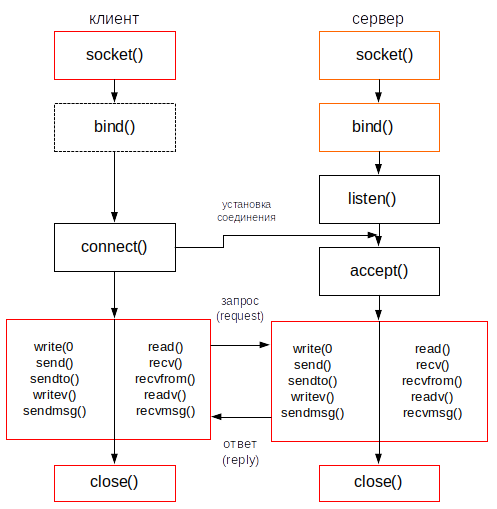
\includegraphics[scale=0.8]{pics/server1.png}}
\end{figure}

Обычно такое взаимодействие выполянется по некоторому протоколу. В сокетах AF\_UNIX взаимодействие ведется через специальный файл, там протокол UDP DEGRAM. 

Протокол - некоторое соглашение, определяющее последовательность действий при взаимодействии, например сервер, получив сообщение, может послать сообщение-подтверждение.

Наша задача - реализовать взаимодействие процессов на отдельно стоящей машине и в распределенной системе. Система с сокетами позволяет моделировать взаимодействие процессов в распределенной системе на отдельно стоящей машине, и мы этим будем пользоваться в нашей ЛР. 

В своей ЛР необходимо запустить несколько процессов-клиентов, и это не fork. Не меньше 3-х клиентов, которые посылают сообщения, например свой ID серверу. Сервер, получив ID, например, выводит его на экран. Нужно ответить еще что-то клиенту. Важно продемонстрировать паралелльность, поэтому запускаем несколько клиентов. Работа ЛР - установление связи и обеспечение обмена сообщениями.

На сокетах определен т.н. сетевой стек. Поскольку у нас две стороны (клиент и сервер), на каждой стороне вызываются свои системные вызовы.

Что-то про стрелочку возле accept. Block until connection from client (accept).

На стороне сервера будет выполняться больше действий. Соединение устанавливается клиентом вызовом connect. 

Вызов bind() используется для назначеня сокету локального адреса. Для сокета интернета этот адрес состоит из ip-адреса сетевого интерфейса локальной системы и номера порта. Клиенты могут не вызывать bind(), т.к. их точный адрес часто не играет никакой роли, при этом адрес назначается им автоматически.

Важный момент: здесь указывается общая струкура sockaddr. Поскольку сокеты декларированы как универсальное средство взаимодействия параллельных процессов, работа на одной локлаьной машине и работа в сети выполняется именно через абстракции конечных точек соединения. На сокетах определено несколько доменов, типов и протоколов, и поэтому на сокетах в самом общем виде определена структура sockaddr. 

\begin{lstlisting}[language=C]
#include <sys/types.h>
#include <sys/socket.h>

int bind(int sockfd, struct sockaddr *addr, int addrlen);

int listen(int sockfd, int backlog);

int connect(int sockfd, struct sockaddr *srvr_addr, int addrlen);

int accept(int sockfd, struct sockaddr *cli_addr, int addrlen);
\end{lstlisting}

Для того, чтобы можно было обеспечивать взаимодействие паралелльных процессов в распределенной системе, определена структура sockaddr\_in, но они сопоставлены друг с другом. И bind, и connect, и accept будут использовать sockaddr, но в программе, если это сетевой сокет, будут инициализироваться поля структуры sockaddr\_in, соотв. функция listen используется сервером чтобы информировать ОС, что процесс-сервер переходит в состояние пассивного ожидания. Соотв. в этом системном вызове 2 параметра - файловый дескриптор, который возвр. socket(), и кол-во прослушиваемых соединений.

Вызов функции listen() имеет смысл только для соединений типа STREAM для протокола TCP.

Функция connect() создает активное соединения клиента с сервером. Должен быть указан адрес сервера.

Вызов accept() - важное действие, соединение может быть принято, если поступил запрос на соединение, иначе принимать нечего. Block until connection from client - процесс будет блокирован на accept(), т.е. очень большую работу выполняет ядро системы. 

Функция accept() используется сервером для принятия соединения при условии, что ранее сервер получил запрос соединения. В противном случае accept() блокируется до получения запроса соединения. При поступлении запроса на соединение, accept() начинает выполняться и создает копию исходного сокета, т.е. получит дескриптор сокета, который был создан функций socket(), а вернет дескриптор нового сокета, который является копией исходного, при этом исходный сокет останется в состоянии listen (будет продолжать прослушивать возникающие соединения), а новый сокет будет находиться в состоянии connected (struct socket.state). 

UNIX/Linux имеют очень тяжелые потоки. Все создается внутри ядра функцией clone(), все зависит от наследования, но между процессами и потоками имеется очень существенная разница - поток выполянется в адресном пространстве процесса, но для UNIX эта декларация весьма условна: системный вызов fork() создает копию процесса-предка, в том смысле, что процесс-потомок наследует код предка.

Мультиплексирование - альтернатива запуска на стороне сервера потоков, каждый из которых обрабатывал бы отдельное соединение.

Пример из книги Стивена, глава 5:

\begin{lstlisting}[language=C]
int main(int argc, char *argv[])
{
	int listenfd, connfd;
	pid_t childpid;
	sock_len_t clilen;
	struct sockaddr_in clientadrr, servadrr;
	listenfd = socket(AF_INET, SOCK_STREAM, 0);
	...
}
\end{lstlisting}

Все системные вызовы нужно проверять на -1.

Адрес апорта получаем из командной строке при запуске на выполнение сервера, но можно присвоить какое-то значение. Номер порта может быть любой. \textit{Порт - это адрес.} 

В наших системах 2 пересекающихся адресных пространства: АП физической памяти и АП портов вода-вывода, при этом размер АП портов ввода-вывода ограничен 64 Кб. Эти АП пересекаются, потому что оба АП начинаются с нулевого адреса. 

А поскольку в системе есть физическая память и есть внешние устройства, которые адресуются через порты, возникает неоднозначность адреса. Чей это адрес - памяти или порта? Поэтому чтобы различать, чей это адрес, исп. т.н. path\_mastering, необходимая составляющая правильной работы ПК (южный и северной мосты).

Многие тенхологии реализуются программно.

АП портов ввода-вывода не преывает 64Кб - использует host to network \textit{short}.

Адрес сокета, номер порта serv\_port - 9877, заранее известен, причем номер порта берется больше, чем 1023, т.к. в этом случае зарезервированный код (порт?) не нужен, порт 9877 для избежания конфликта с динамическими портами. пассивное прослушивание - основную работу на себя берет система. Сервер блокируется на вызове accept в ожидании соединения с клиентом. Для каждого клиента функция fork создает процесс-потомок для обслуживания клиента, при этом процесс-потомок закрывает прослушивающий сокет, а в процессе-предке сокет остается прослушивающим. Так можно сделать, потому что это другой процесс. Затем вызывается функция str\_echo для обработки запроса клиента. Можно сделать на коленке: recvfrom, sendto.

Пример - показать, альтернативой чему является мультиплексирование. Каждое соединение обслуживается отдельным процессом.

\section{Мультиплексирование ввода-вывода}

2 основных мультиплексера. Родным для UNIX BDS является select, для system5 - multiplexing pool. Есть select, есть pselect, но если последний параметр (sigmask) pselect установить в NULL, будет тот же самый select. Очень хорошо описан select, pool описан хуже, но он лучше. Каждый из мультиплексеров определен в системе.

Рассмотрим пример: сервер обслуживает какое-то кол-во соединений и ожидает сообщение от любого соединения. В этом случае нельзя использовать блокирующую операцию чтения, т.к. чтение одного дескриптора приведет к блокировке программы, в ожидании когда данные смогут быть прочитаны, в это же время данные могут появиться на других соединениях (на другом дескрипторе). 

Для решения этой проблемы используется мультиплексирование ввода-вывода. Для этого необходимо создать список (массив) дескрипторов и вызвать мультиплексер, который мультиплексирует соединения (мультиплексер блокирует процесс до появления \textit{любого} первого соединения) и вернет управление. При выходе из функции мультиплексирования сервер получит информацию о готовых к вводу-выводу дескрипторах.

Мультиплексер select определен в posix.1, поэтому он лучше описан.

Если мы работаем с мультиплексером, необходимо объявить массив дескрипторов, потому что этот массив будет заполнен и в последствии работа будет выполняться с массивом дескрипторов.

\begin{lstlisting}[language=C]
int select(int h, fd_set *readfds, fd_set *write_fds, fd_set *exceptfds, struct timeval *timeout);

//functions defined on SELECT
FD_CLR(int fd, fd_set *set);

FD_ISSET(int fd, fd_set *set); // do descr is a part of select?
\end{lstlisting}

Выстанавливается timeout, чтобы не ждать бесконечно.

\chapter{\textbf{Лекция 4 июня 2022}}

\section{Специальные файлы устройств.}

Эти файлы обеспечивают унифицированный доступ к внешним устройствам или перефирии. Эти файли обеспечивают связь файловой системы и драйверов устройств.

Такая интепретация специальных файлов устройств обеспечивает доступ к внешним устройствам как к обычным файлам. Также как и обычные файлы, файл устройства может быть открыт, закрыт, из него можно читать или в него можно писать. 

Каждому внешнему устройству UNIX и Linux ставит в соответствие как минимум один специальный файл. Обычно эти файлы можно увидеть в каталоге /dev (первая буква c - character, b - block) корневой файловой системы. Подкаталог /dev/fd содержит файлы с именами 0, 1, 2, но в некоторых системах имеются файлы с именами /dev/stdin, и соответственно /stdout, /stderr.

Система поддерживает 2 типа специальных файлов устройства: \textit{символьный }(небуферизуемый, non buffered) и \textit{блочный} (буферизуемый). В UNIX/Linux связь имени специального файла с конкретным внешним устройством обеспечивает inode, или индексный дескриптор.

Взаимодействие прикладных программ с аппаратной частью ПК под управлением ОС UNIX/Linux осуществляется по следующей схеме:

\begin{figure}[!h]
	\center{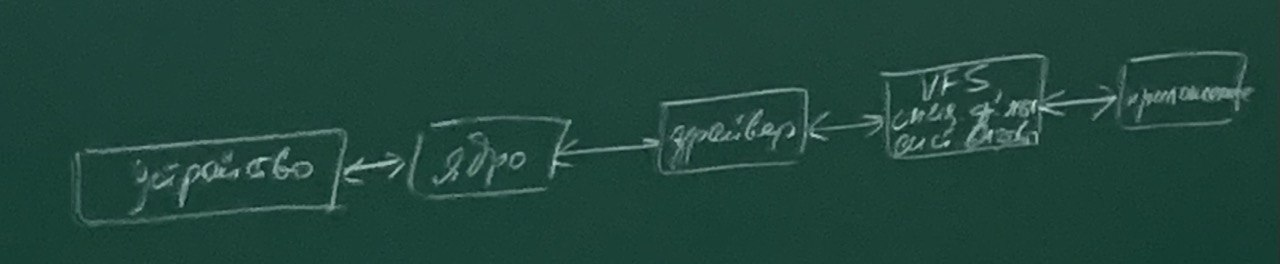
\includegraphics[scale=0.4]{pics/driver.jpg}}
\end{figure}

Драйвер - часть кода ядра, которая предназначена для управления конкретным устройством. Драйверы в любой системе пишутся по правилам этой системы на основании структур ядра, определенных в системе. Такие структуры перечисляют точки входа в драйвер и другие параметры, т.е. драйвер - не произвольно написанный код, он написан по жестким правилам системы, но задача драйвера - управлять внешним устройством.

Драйвер должен преобразовывать данные поступающие на устроство, получаемые от утсройства. Если драйверу нужно передать данные устройству, их нужно передать в формате данных, определенном на устройстве. Когда данные получаются, в итоге формат данных, полученный от устройства, должен быть преобразован в формат, понятный приложению.

В Windows определен т.н. стек драйверов. Внести функциональность в Windows можно только с помощью драйвера. Только разработчик устройства знает все передаваемые параметры.

Драйверы устройств в UNIX/Linux бывают 3 типов:

\begin{itemize}
	\item Встроенные драйверы - их выполнение инициализируется при запуске системы. Пример таких устройств: VGA-контроллер, контроллеры IDE, материанская плата, последовательные и параллельные порты;
	\item Драйвера, реализованные как загружаемые модули ядра - часто используются для управления SCSI-адаптерами, звуковыми и сетевыми картами. Файлы модуля ядра располагаются в подкаталогах каталога /lib/modules. Обычно при инсталляции системы задается перечень модулей, которые будут автоматически загружаться при этапе загрузки. Список загружаемых модулей хранится в /etc/modules, в файле /etc/modules.conf находится перечень опций. Для досупа к ним существуют специальные скрипты типа update-modules. Для подключения или отключения модулей в работающей системе имеются специальные утилиты (команды) - lsmod, insmod, rmmod, modprop (автоматически загружает модули; чтобы отобразить текущую конфигурацию всех модулей нужно воспользоваться командной modprop -c);
	\item Код драйверов 3 типа поделен между ядром и специальной утилитой, например у драйвера принтера ядро отвечает за взаимодействие с параллельным портом, а формирование управляющих сигналов для принтера осуществляет демон печати lpd, который для этого использует специальную программу-фильтер.
\end{itemize}

Хит-драйвера (хьюман интерфейс) - мышь, клавиатура, обеспечивают взаимодествие с пользователем.

В системе имеются старший (major, основной) или младший (minor, дополнительный) номера драйвера устройств. Это общий подход к идентификации как символьных, так и блочных устройств. Для примера рассмотрим символьные устройства. Блочными устройствами системы являются внешние запоминающие устройства, остальные - символьные (последовательный ввод).

Рассмотрим пример. 

\begin{lstlisting}[language=C]
$ cd dev
$ ls -l
crw-rw-rw- 1 root root 1,  3  <data> null
crw------- 1 root root 10, 1  <data> psaux
crw------- 1 root root 4,  1  <data> tty1
crw-rw-rw- 1 root tty  4, 64  <data> tty0
...
crw-rw-rw- 1 root root 1,  5  <data> zero
\end{lstlisting}

2 числа через запятую - номера устройств. Традиционно старший и младший номер идентифицируют драйвер, который связан с устройством, например /dev/null и /dev/zero управляются драйвером 1, а виртуальные консоли и последовательные терминалы управляются драйвером 4.

Современное ядро Linux позволяет множеству драйверов разделять старшие номера, но большинство устройств, которые можно увидеть в/dev, все еще организованы по принципу один старший - один драйвер. Младшие номера используются ядром для определения конкретного устройства. 

Внутреннее представление номеров устройств: в ядре существует тип dev\_t.

Стандарт posix.1 определяет существование этого типа, но не определяет формат полей. Тип определен в <linux/types.h>. Начиная с версии ядра 2.6.0 dev\_t - 32-разрядное число, в котором 12 бит отведены для старшего номера и 20 для младшего. 

Это важно при написании собственного драйвера устройства, при этом код драйвера никак не должен интерпретировать эти значения, он должен их просто использовать. Для этого необходимо использовать набор макросов из <linux/kdev\_t.h>. Эти макросы позволяют получить старший и младший номера устройств.

\begin{lstlisting}[language=C]
MAJOR(dev_t dev);
MINOR(dev_t dev);
\end{lstlisting}

Также возможны обратные действия - преобразования номеров в dev\_t:

\begin{lstlisting}[language=C]
MKDEV(int major, int minor)
\end{lstlisting}

Исходя из формата, можно сказать, что начиная с ядра 2.6, система может поддерживать огромное число номеров устройств, в отличие от ядер предыдущего поколения, которые имели ограничения для старших и младших номеров по 255 штук.

Выделение и освобождение номеров устройств: одно из первых действий драйвера, когда устанавливается символьно устройство - получение одного и более номеров устройств.

Для того, чтобы драйвер получил старший и младший номера:
\begin{lstlisting}[language=C]
#include <linux/fs.h>

int register_chrdev_region(dev_t first, unsigned int count, char *name);
\end{lstlisting}

Часть minor часто устанавливается в 0, но никаких требований нет. Count - количество номеров устройств, которые запрашиваются. Если count больше, чем диапазон, который запрашивается, то может случиться переход через диапазон на следующий старший номер, но все будет работать нормально до тех пор, пока будет доступен запршиваемый диапазон номеров. Имя устройства, которое связывается с диапазоном номеров, можно увидеть в /proc/devices и /sys/fs.

Данная функция хорошо работает, если заранее известно конкретное устройство, которому нужен номер, однако часто неизвестно, какой старший номер использует ваше устройство, поэтому разработчики ядра особо подчеркивают, что для динамического выделения старшего номера нужно использовать следующую функцию:

\begin{lstlisting}[language=C]
int alloc_chrdev_region(dev_t dev, unsigned int firstminor, 
															unsigned int count, char *name);
\end{lstlisting}

В этой функции параметр dev - только выходной, и он будет содержать первый номер в выделенном диапазоне при успешном завершении вызова функции. Firstminor - первый запрошенный младший номер, обычно равен 0. Count и name - параметры, аналогичные первой функции.

Несмотря на то, как выполняется рапсределение номеров устройств в вашем драйвере, необходимо их освободить, когда они больше не используются. Для этого вызывается следующая функция:

\begin{lstlisting}[language=C]
void unregister_chrdev_region(dev_t first, unsigned int count);
\end{lstlisting}

Обычно эта функция вызывается exit() или cleanup(), alloc - в init().

Динамическое выделение старшего номера: некоторые старшие номера статически назначаются большинству обычных устройств. Для того, чтобы посмотреть такие старшие номера, уже используемые в текущей реализации Linux, надо посмотреть /proc/devices.

С помощью команды \textbf{ls -l /dev/ | grep "\^c"} мы получим список символьных файлов устройств в системе. 

Обычно в системе существует уже хорошо известный набор старших драйверов(?58м):

\begin{figure}[!h]
	\center{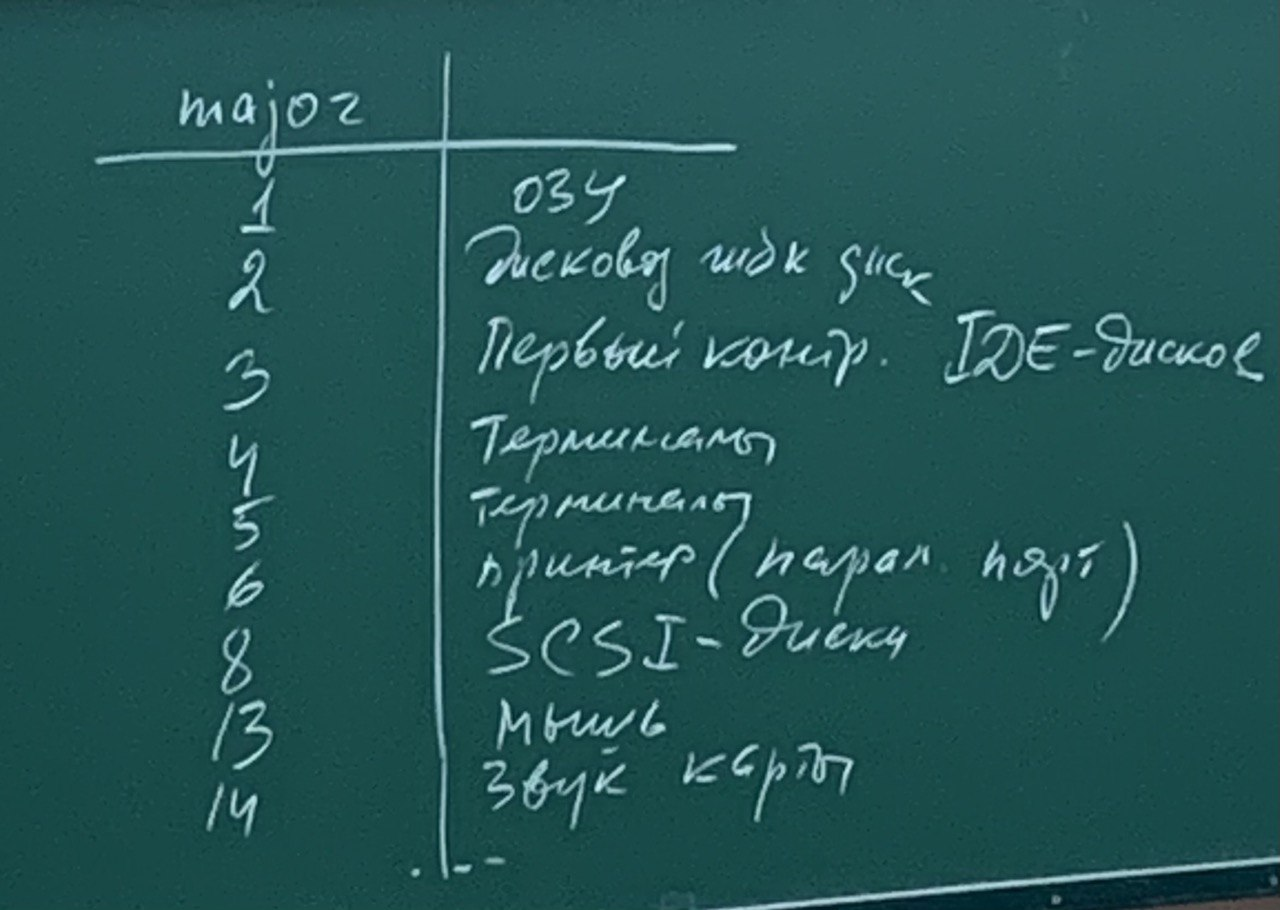
\includegraphics[scale=0.35]{pics/driver2.jpg}}
\end{figure}

Ориентируясь на выделенные в системе старшие номера, можно выбрать старший номер для своего драйвера. Кроме того, могут быть назначены случайные статические номера, но при этом новые номера не присваиваются. В результате разработчик драйвера должен сделать вывод: можно просто подобрать номер, который кажется неиспользуемым, или выделить старшие номера динамически.

Подобранный номер может работать так долго, как долго вы сами будете пользоваться собственным драйвером. Как только ваш драйвер получит более широкое распространение, случайно выбранный старший номер скорее всего приведет к конфликтам и неисправности. Таким образом, разработчики ядра настоятельно рекомендут использовать динамическое получение старших номеров устройства. 

У динамического выделения имеется недостаток: нельзя заранее создать узлы устройства, т.к. главный номер будет получен в последствии, т.е. он неизвестен. Существуют рекомендации, одна из них - при загрузке драйвера с динамическим назначением старшего номера вызов insmod следует заменить соответствующим скриптом, который после вызова insmod будет читать /proc/devices/, чтобы создать специальный файл/файлы. 

Рекомендуется в скрипте использовать инструмент типа awk. Команда awk читает документ по строкам и выполняет указанные разработчиком действия, результат выводит на stdin.

\begin{lstlisting}[language=C]
$ awk options 'condition{action}' //Example
major = $(awk "\\$2 = = \"$module" {print \\$1}")proc/devices.
\end{lstlisting}

Функция register\_chrdev\_region() используется для статического выделения. Для динамического надо использовать alloc\_chrdev\_region() и соотв. скрипт.

Драйвер устройства содержит такие функции, как open, close, read, write, и эти функции должны быть определены для вашего драйвера. Здесь работает все, что было рассмотрено в курсе 2 семестра: моедли, передеча данных UK-KU.

Основная часть драйверов в качестве одной из точек входа имеет обработчик аппаратного прерывания. Если нужно дополнительно обработать данные, поступаемые в результате работы обработчика прерывания, используются тасклеты и очереди работ.

В ядре имеется набор структур, определенных для работы с внешними устройствами. Основной структурой является struct device. Эта структура нижнего уровня, но поля этой структуры инициализируются при включении конкретного устройства. Расмотрим некоторые поля.

\begin{lstlisting}[language=C]
struct device {
	struct device *parent;
	...
	const char *init_name;
	...
	struct bus_type *bus;
	struct device_driver *driver;
	...
	struct dma_coherent_mem *dma_mem;
	...
};
\end{lstlisting}

Устройство может не иметь родительского устройства. Такое устройство - top level. Первоначальное имя устройства - init\_name. Для любого устройства важно, к какой шине оно подключается.

Direct memory access - способ освобождения процессора от рутинной перекачки данных от устройства в оперативную память. (1.19м)

Установка поля coherent DMA mapping API - установка устойчивых соединений многократно использумых буферов. Нет необходимости предварительно выделять буфер dma.

dev\_t поле для создания в <sys/fs> устройства. u32 id - экземпляр устройства.

driver - основная структура, описывающая драйвер.

\begin{lstlisting}[language=C]
struct driver {
	const char *name;
	struct bus_type *bus;
	struct module *owner;
	...
	int (*probe)(struct device *dev);
	int (*remove)(struct device *dev);
	...
	int (*resume)(struct device *dev);
	...
};
\end{lstlisting}

\end{document}